\newpage
\section{几何先验}
\label{sec:geom_priors}
现代数据分析几乎等同于高维学习。
尽管第~\ref{sec:inductive} 节中的简单论证表明，由于维数灾难，不可能从一般高维数据中学习，
但对于具有物理结构的数据仍有希望，因为我们可以采用两条基本原则：{\em 对称性}与{\em 尺度分离}。
在本文所考虑的设置中，这种附加结构通常来自输入信号底层域的结构：
我们将假设机器学习系统作用于某个域 $\Omega$ 上的\emph{信号}（函数）。
%
尽管在许多情况下，$\Omega$ 上点的线性组合并没有良好定义\marginnote{$\Omega$ 必须是向量空间，表达式 $\alpha u + \beta v$ 才有意义。}，但我们可以对其上的信号作线性组合；也就是说，信号空间构成一个向量空间。
此外，由于可以定义信号之间的内积，该空间是一个{\em Hilbert 空间}。

\begin{tcolorbox}[width=\linewidth,
                  boxsep=0pt,
                  left=7.5pt,
                  right=7.5pt,
                  top=7.5pt,
                  bottom=7.5pt,
                  arc=0pt,
                  boxrule=0pt,toprule=0pt,
                  colback=boxgray,
                  ]%%

取值于 $\mathcal{C}$、定义在 $\Omega$ 上的信号空间
\marginnote{当 $\Omega$ 具有某种附加结构时，可以进一步限制 $\mathcal{X}(\Omega, \mathcal{C})$ 中信号的类型。例如，当 $\Omega$ 是光滑流形时，可以要求信号光滑。
为简洁起见，只要不会引起歧义，我们将省略值域 $\mathcal{C}$。
} %can impose smoothness on the signals.}% For instance, when $\Omega$ is a smooth manifold we may require signals in $\mathcal{X}(\Omega, \mathcal{C})$ to be smooth.}
（其中 $\Omega$ 是一个可能具有附加结构的集合，$\mathcal{C}$ 是一个向量空间，其维度称为\emph{通道}）
\begin{equation}
    \mathcal{X}(\Omega, \mathcal{C}) = \{ x : \Omega \rightarrow \mathcal{C} \}
\end{equation}
%
是一个具有向量空间结构的函数空间。
%In particular, it satisfies the distributivity property 
信号的加法与标量乘法定义为：
\begin{equation*}
    (\alpha x + \beta y)(u) = \alpha x(u) + \beta y(u) \quad \text{for all} \quad u\in \Omega,
\end{equation*}
其中 $\alpha, \beta$ 为实标量。% are vectors, and $u \in \Omega$.
%
给定内积 $\langle v, w \rangle_\mathcal{C}$（定义在 $\mathcal{C}$ 上）以及测度\marginnote{当域 $\Omega$ 是离散的时，可以选择 $\mu$ 为{\em 计数测度}，此时积分变为求和。下文将省略测度，并为简洁起见使用 $\mathrm{d}u$。}$\mu$（定义在 $\Omega$ 上，并可据此定义积分），就可以在 $\mathcal{X}(\Omega, \mathcal{C})$ 上定义如下内积：
\begin{equation}
    \langle x, y \rangle = \int_{\Omega} \langle x(u), \, y(u) \rangle_{\mathcal{C}} \; \mathrm{d}\mu(u).
    \label{eqn:innerprod}
\end{equation}
\end{tcolorbox}

%we will assume that $f$ operates on $\mathcal{C}$-valued signals $\mathcal{X}(\Omega, \mathcal{C}) = \{x: \Omega \rightarrow \mathcal{C} \}$, where $\Omega$ is some input domain and $\mathcal{C}$ is a vector space, typically $\mathcal{C} = \R^s$ for a signal with $s$ channels.
%\marginnote{For the sake of simplicity, we will often assume scalar-valued signals, i.e., $s=1$. }
%We note that $\mathcal{X}(\Omega, \mathcal{C})$ is a vector space, with addition and scalar multiplication defined pointwise (i.e. $(f + f')(x) = f(x) + f(x')$ and $(\alpha f)(x) = \alpha f(x)$).

作为一个典型示例，令 $\Omega = \mathbb{Z}_n\times \mathbb{Z}_n$ 为二维 $n\times n$ 网格，令 $x$ 为 RGB 图像（即信号 $x : \Omega \rightarrow \R^3$），并令 $f$ 为作用于 $3n^2$ 维输入的函数（例如单层感知机）。
%
正如下文将更详细说明的，域 $\Omega$ 通常配备某种几何结构与对称性。%symmetric structure (in our example, rotational and translational symmetry) that is manifested both in signals $x$ defined on this domain as well as in functions $f$ acting on such signals.
%
尺度分离源于这样一种能力：把信号转移到较粗糙版本的域上时，仍能保留信号的重要特征（在本例中，即通过粗化底层网格对图像进行下采样）。


我们将说明，这两条原则——统称为{\em 几何先验}——在多数现代深度学习架构中都十分突出。对于上述图像情形，几何先验通过共享权重的卷积滤波器（利用平移对称性）和池化（利用尺度分离）被内置于卷积神经网络（CNN）中。
%
把这些思想推广到图、流形等其他域，并说明几何先验如何从基本原则中产生，是几何深度学习的主要目标，也是本文的{\em 主旋律}。



\subsection{对称性、表示与不变性}
\label{sec:symmetries}

%Symmetries are a foundational principle of physics, providing a strong constraint on the form of physical laws.
%In the context of machine learning, symmetries also provide key regularity priors that allow to break the curse of dimensionality and enable efficient high-dimensional learning. 

非正式地说，对象或系统的{\em 对称性}是一种使该对象或系统的某种性质保持不变，即保持{\em 不变性}的变换。
这类变换可以是光滑的、连续的或离散的。
%A canonical example for continuous symmetries in physics is Lagrangian mechanics, which states that the laws of motion are preserved under rigid transformations of the observer's point of view. 
%
对称性普遍存在于许多机器学习任务中。
例如，在计算机视觉中，物体类别不随平移而改变，因此平移是视觉物体分类问题中的对称性。
%one is often interested in classifying  objects in images independently of their position, a setting referred to as {\em translation invariant}. 
%
%classification through translation invariance, or 
在计算化学中，要在不依赖分子空间取向的情况下预测分子性质，需要{\em{旋转不变性}}。
%
在描述粒子没有典范次序、因而可以任意置换的粒子系统时，离散对称性会自然出现；在许多动力系统中，离散对称性也会通过时间反演对称性自然出现
%through permutations, 
%or also 
（例如满足细致平衡的系统或 Newton 第二运动定律）。%\marginnote{ADD COMMENT on Newton's law} % may not be necessary imo
%
正如第~\ref{sec:proto-graphs} 节将看到的，置换对称性也是分析图结构数据的核心。% and will be a prominent topic in this book.

\paragraph{对称群}
一个对象的对称性集合满足若干性质。
%which make this set into an algebraic structure called a \emph{symmetry group}.
%Symmetries lend themselves to a rich and powerful mathematical characterization.
%More specifically, the set of symmetries of a given object forms an algebraic object called a symmetry group.
首先，可以组合对称性来得到新的对称性：如果 $\fg$ 和 $\fh$ 是两个对称性，
%transformations of a system that leave it unchanged, 
那么它们的复合 $\fg \circ \fh$ 和 $\fh \circ \fg$
%\marginnote{From hereon we will denote composition of group elements by $\fg \fh$, leaving out the $\circ$ symbol.}
\marginnote{我们将遵循群论中使用的并置记号约定 $\fg \circ \fh = \fg \fh$；它应从右向左读，即先应用 $\fh$，再应用 $\fg$。次序十分重要，因为许多情况下对称性不满足交换律。
%
熟悉 Lie 群的读者可能会对我们使用 Fraktur 字体表示群元素感到不习惯，因为这种字体通常用于表示 Lie 代数。
}也仍然是对称性。
原因在于，如果两个变换都使对象保持不变，那么它们的复合也具有这一性质，因此该复合仍是对称性。
%\marginnote{This property is called {\em closure} in group theory.} 
此外，对称性总是可逆的，并且其逆仍是对称性。
%Together with {\em associativity} $(\fg \circ \fh) \circ \ff = \fg \circ (\fh \circ \ff)$ of the composition operation and existence of unique {\em identity} ($\exists!\fe \in \fG$ such that $\fe \circ \fg = \fg \circ \fe = \fe$ for all $\fg \in \fG$) and {\em inverse} (for any $\fg \in \fG$, $\exists! \fg^{-1} \in \fG$ such that $\fg\circ \fg^{-1} = \fg^{-1}\circ \fg = \fe$), it formally defines a group.} 
这表明，所有对称性的集合构成一个称为{\em 群}的代数对象。由于这类对象将成为几何深度学习数学模型的核心，因此有必要给出正式定义并作详细讨论：
%The symmetries of any system thus form a {\em group} with the composition operation, which can be studied with powerful tools from representation theory, algebra and geometry.


%\taco{TODO: Make this into a Definition Box.}


\begin{tcolorbox}[width=\linewidth,
                  boxsep=0pt,
                  left=7.5pt,
                  right=7.5pt,
                  top=7.5pt,
                  bottom=7.5pt,
                  arc=0pt,
                  boxrule=0pt,toprule=0pt,
                  colback=boxgray,
                  ]%%
{\em 群}是一个集合 $\fG$，并配备称为{\em 复合}的二元运算 $\circ : \fG \times \fG \rightarrow \fG$（为简洁起见，用并置 $\fg \circ \fh = \fg \fh$ 表示）
%for $\fg, \fh \in \fG$, 
且满足以下公理：\vspace{3mm}\\
%\begin{enumerate}
    %\item 
    \noindent {\em 结合律：}$(\fg \fh) \fk = \fg (\fh \fk)$ 对所有 $\fg, \fh, \fk \in \fG$ 成立。\vspace{2mm}\\
    \noindent  {\em 单位元：}存在唯一的 $\fe \in \fG$，满足 $\fe \fg = \fg \fe = \fg$，且这一条件对所有 $\fg \in \fG$ 成立。\vspace{2mm}\\
    \noindent  {\em 逆元：}对每个 $\fg \in \fG$，都存在唯一的逆元 $\fg^{-1} \in \fG$，使得 $\fg \fg^{-1} = \fg^{-1} \fg = \fe$。\vspace{2mm}\\
    \noindent  {\em 封闭性：}群对复合运算封闭，即对每个 $\fg, \fh \in \fG$，都有 $\fg \fh \ \in \fG$。
%\end{enumerate}

\end{tcolorbox}
注意，\emph{交换律}并不是该定义的一部分，即可能有 $\fg \fh \neq \fh \fg$。
若一个群满足 $\fg \fh = \fh \fg$，且这一条件对所有 $\fg, \fh \in \fG$ 成立，则称其为交换群或{\em Abel 群}\marginnote{该名称源自挪威数学家 Niels Henrik Abel（1802--1829）。}。

尽管有些群可能非常大，甚至是无限群，但它们通常可以由少数几个元素复合产生，这些元素称为{\em 群生成元}。形式上，称 $\mathfrak{G}$ 由子集 $S \subseteq \mathfrak{G}$ {\em 生成}（该子集称为群的{\em 生成元}），如果每个元素 $\fg \in \fG$ 都可以写成 $S$ 中元素及其逆元的有限复合。
%
例如，等边三角形的对称群（二面体群 $\mathrm{D}_3$）由一个 $60^\circ$ 旋转和一个反射生成（图 \ref{fig:group-example-d3-s3}）。
%
下文将详细讨论的一维{\em 平移群}由无穷小位移生成；这是可微对称性的{\em Lie 群}实例。\marginnote{Lie 群具有可微流形结构。第~\ref{sec:groups} 节将研究的特殊正交群 $\mathrm{SO}(3)$ 就是一个例子，它是三维流形。}


注意，这里把群定义为一个抽象对象，并未说明群元素\emph{是什么}（例如某个域的变换），只说明它们如何\emph{复合}。
因此，类型迥异的对象可能具有相同的对称群。
例如，前述三角形旋转与反射对称群，和三个元素序列的置换群相同（利用旋转与反射可以任意置换三角形的顶点——见图 \ref{fig:group-example-d3-s3}）\marginnote{图 \ref{fig:group-example-d3-s3} 所示图形（每个节点对应一个群元素，每条箭头对应一个生成元）称为{\em Cayley 图}。}。

\begin{figure}
    \centering
\raisebox{-0.5\height}{    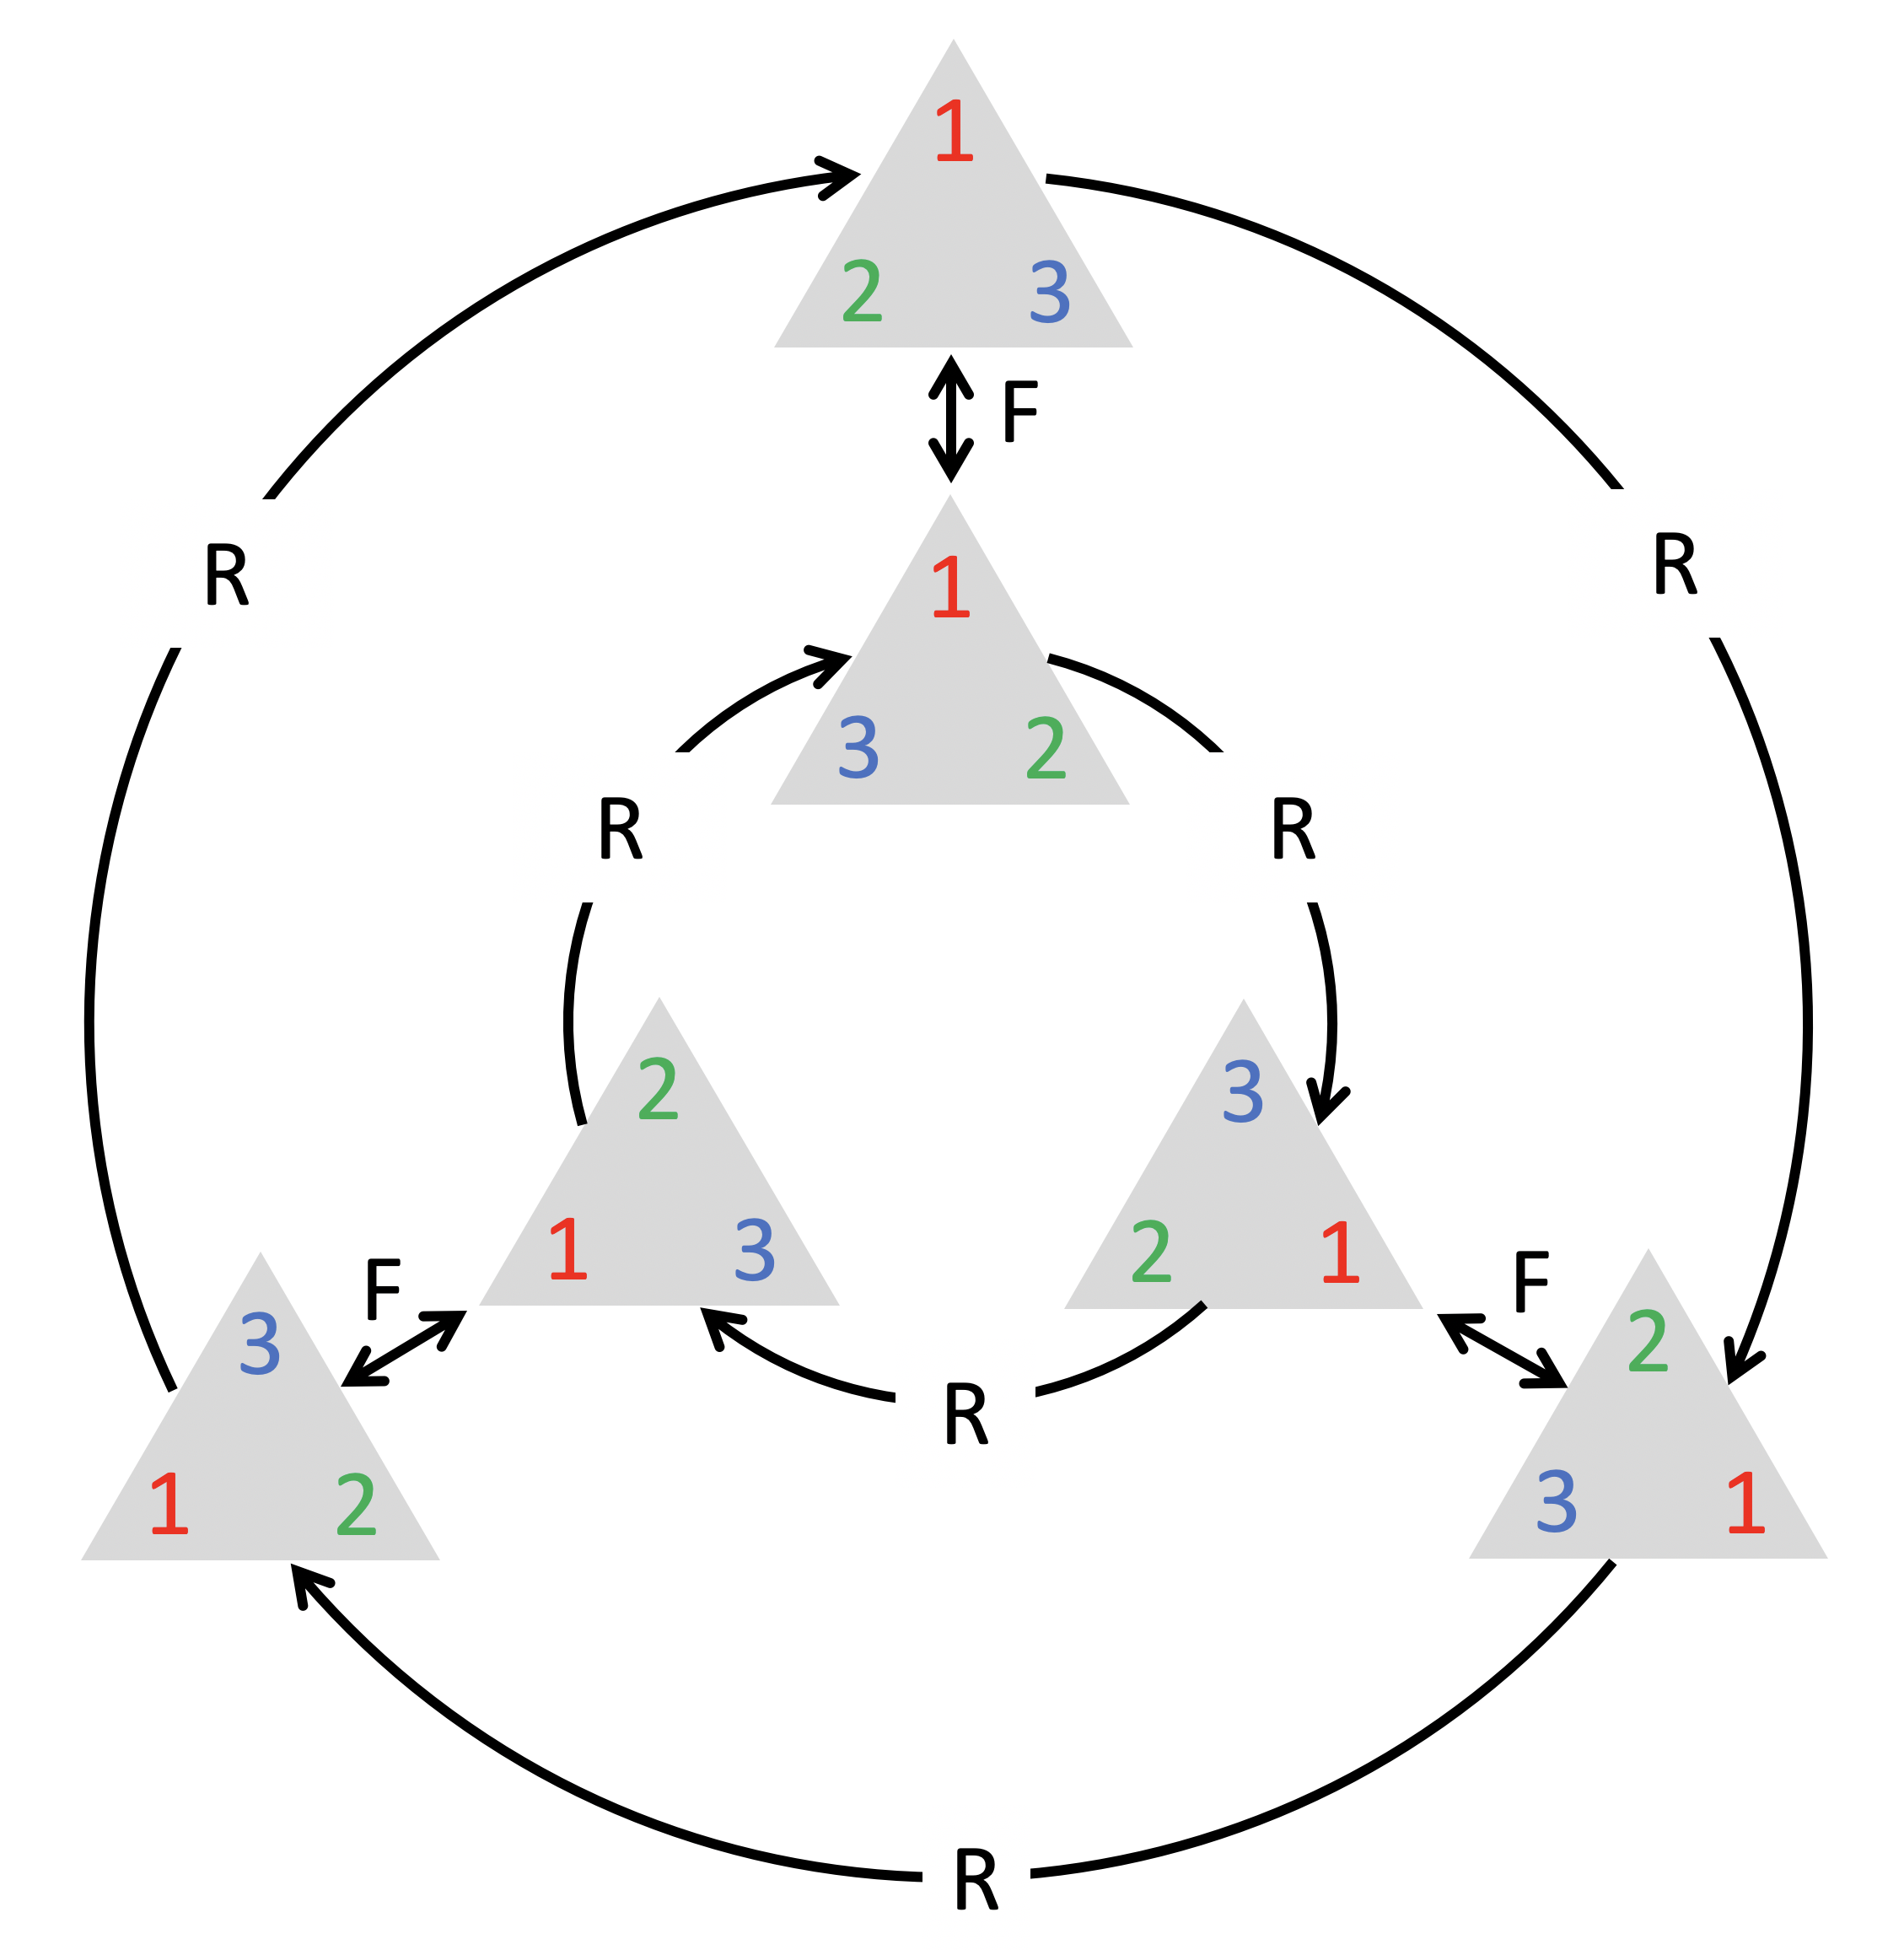
\includegraphics[width=0.45\linewidth]{figures/group_d3.png}
}
    \hspace{2mm}
    \raisebox{-0.5\height}{
        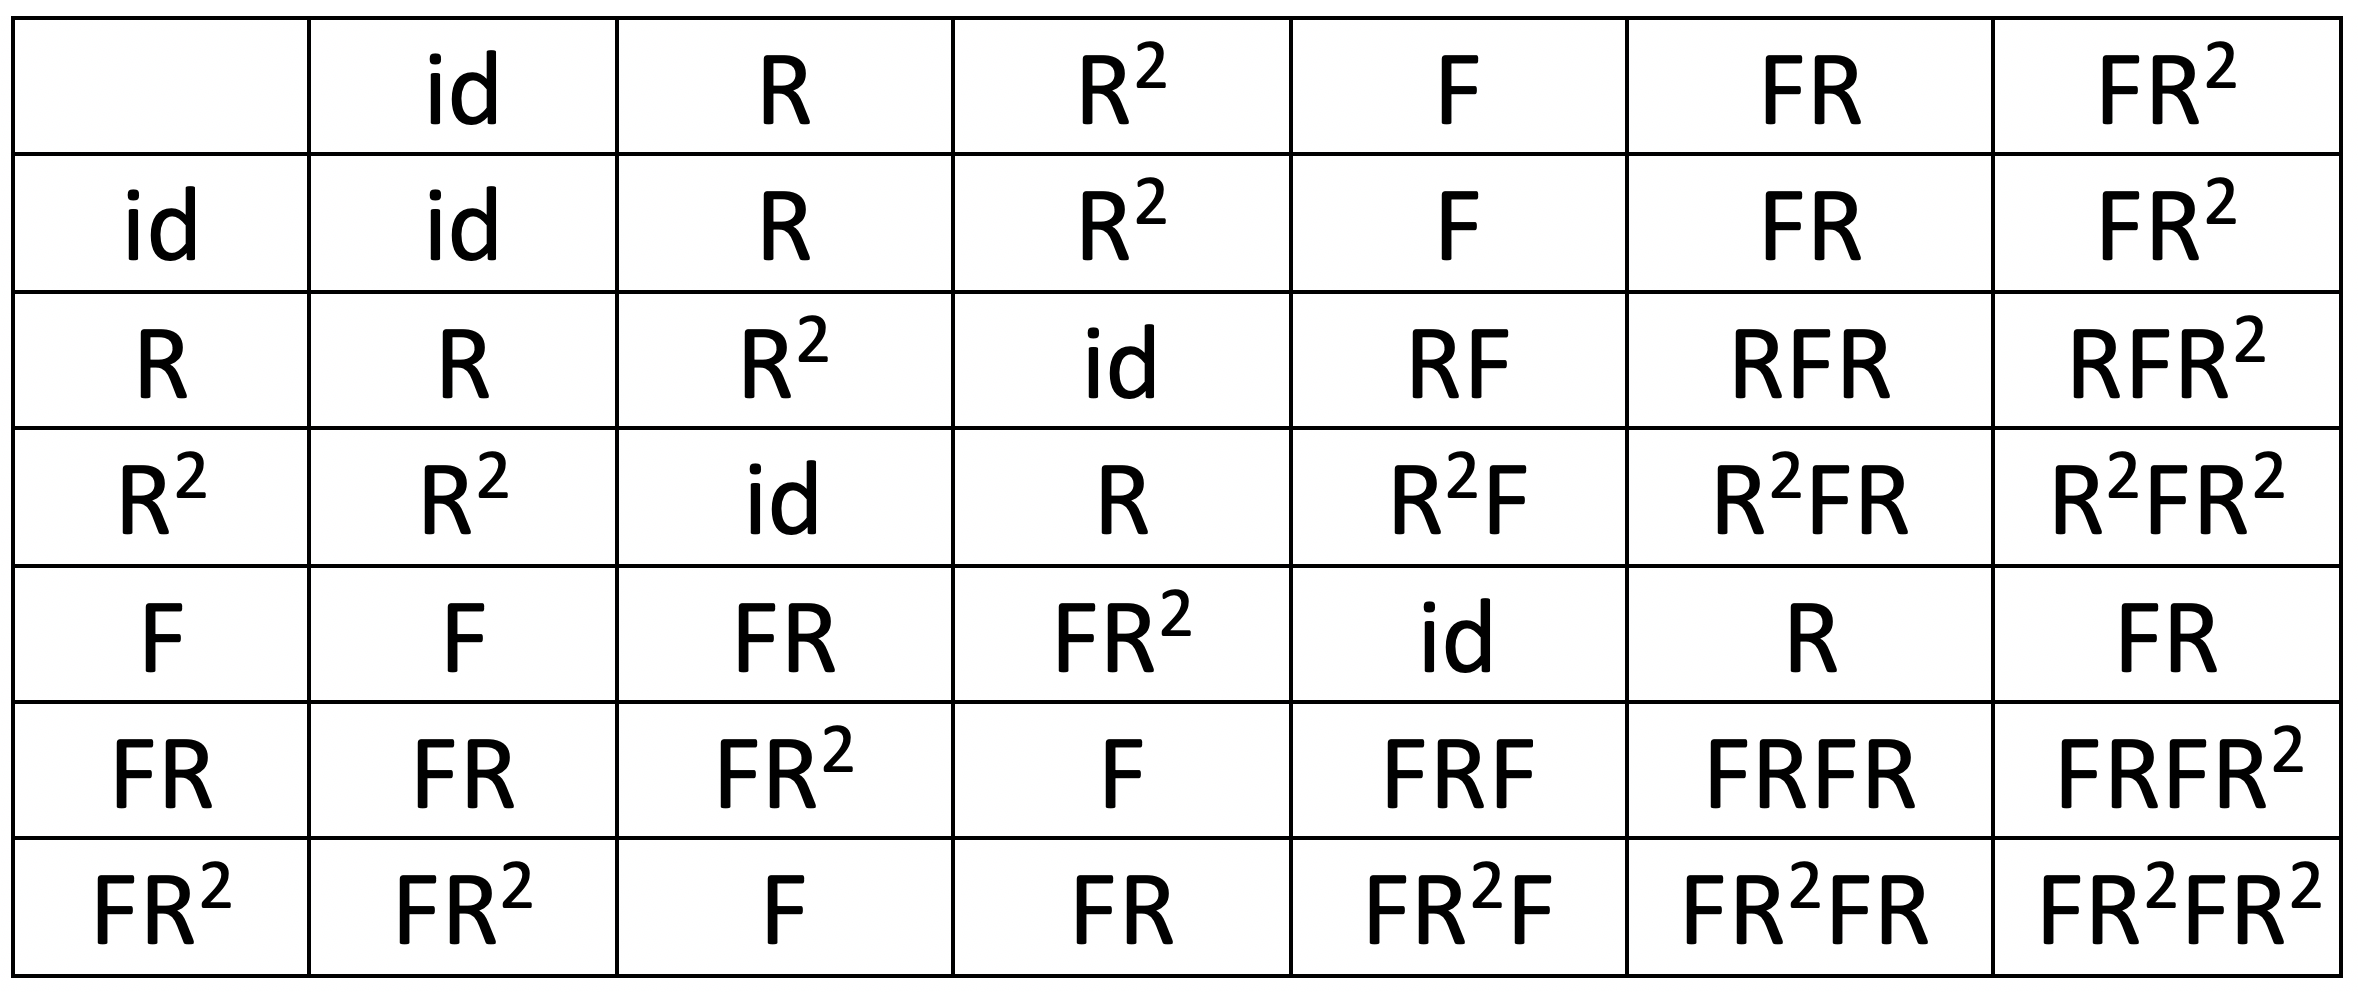
\includegraphics[width=0.48\linewidth]{figures/group_d3_m.png}
        }
%    \taco{TODO: figure of a triangle with labelled corners (0,1,2), and all permutations of it, as a Cayley diagram. Could add multiplication table of the group as well.}
    \caption{左：顶点标记为 $1, 2, 3$ 的等边三角形，以及该三角形所有可能的旋转与反射。三角形的旋转/反射对称群 $\mathrm{D}_3$ 仅由两个元素生成（旋转 $60^\circ$ 的 R 和反射 F），并且与三个元素的置换群 $\Sigma_3$ 相同。
    右：群 $\mathrm{D}_3$ 的乘法表。第 $\fg$ 行、第 $\fh$ 列的元素对应元素 $\fg \fh$。%\taco{\bf TODO: We need to reverse the Rotation arrows on the outer (or inner) ring. All rotations should be either clockwise or counter-clockwise}}
    \label{fig:group-example-d3-s3}
    }
\end{figure}

% Note that this definition provides a self-consistent description of a standalone object that is the main focus of study in group theory. Despite its apparent simplicity, this theory is rich with many deep results. 
% %despite the apparent simplicity of its basic definition.
% %
% %
% In geometry, key insights are obtained when transformations on a domain are modelled as elements of a group and the group theory formalism is used to study their properties --- this was exactly the breakthrough idea of Klein we have mentioned in the beginning of our discussion. 
% %
% %The way in which elements of symmetry groups act on points on a domain provides important insights about the structure of such domain --- 
% %
% %Group theory is a very rich area with many deep results, despite the apparent simplicity of its basic definition. 
% %
% %symmetry groups turn out to have rich internal algebraic structure with fascinating mathematical properties. 

\paragraph{群作用与群表示}
%
与其把群视为抽象实体，
我们更关心群如何\emph{作用}于数据。
%The structure of such groups reveals the symmetry concealed in the data, which in turn leads to powerful geometric priors. 
%
%The assumption In geometric deep learning, one typically starts 
由于我们假设数据以某个域 $\Omega$ 为基础，因此将研究群如何作用于 $\Omega$
（例如平面上点的平移），并由此得到同一个群在信号空间 $\mathcal{X}(\Omega)$ 上的作用
%\marginnote{Whenever possible, we will omit the range $\mathcal{C}$ for brevity.} %in which our data lives 
（例如平面图像与特征图的平移）。


% Taco: I am commenting this here, because 1) I think the notion of automorphism should be introduced differently. An auto is an iso from an object to itself. The meaning of iso depends on the context (category), i.e. on what properties/structure we wish to preserve. So when we introduce autos and subgroups, we should just say that we can preserve more or less structure, and get smaller or larger groups. 2) I think here the flow is disrupted a bit, and it would fit better in the deformation section.

% First, let us consider a broad class of bijective domain transformations called {\em automorphisms}
% $$\mathrm{Aut}(\Omega) = \{ \tau: \Omega \xrightarrow{1:1} \Omega \}.$$ 
% %
% Automorphisms also form a group with the composition operation. 
% %
% We can consider symmetries as `subsets' of automorphisms that preserve some structure: for example, in the plane the {\em Euclidean group} $\mathrm{E}(2)$ is the group of transformations of $\R^2$ that preserves Euclidean distances\marginnote{Distance-preserving transformations are called {\em isometries}. According to Klein's Erlangen Programme, the classical Euclidean geometry arises from this group.}, and consists of translations, rotations, and reflections.
% %
% More formally, a symmetry group $\fG$ constitutes a {\em subgroup} of the automorphism group $\mathrm{Aut}(\Omega)$: 

% \begin{tcolorbox}[width=\linewidth,
%                   boxsep=0pt,
%                   left=7.5pt,
%                   right=7.5pt,
%                   top=7.5pt,
%                   bottom=7.5pt,
%                   arc=0pt,
%                   boxrule=0pt,toprule=0pt,
%                   colback=boxgray,
%                   ]%%
% Let $(\fG,\circ)$ be a group and $\mathfrak{H} \subseteq \fG$ a subset. $\mathfrak{H}$ is said to be a {\em subgroup} of $\fG$ if $(\mathfrak{H},\circ)$ constitutes a group with the same operation. 
% \end{tcolorbox}


%we have considered so far are subgroups of $\mathrm{Aut}(\Omega)$. \marginnote{A subset $\fG \subseteq \frak{H}$ is said to be a {\em subgroup} of a group $(\frak{H}, \circ)$ if it forms a group $(\frak{G}, \circ)$ with the same operation.}



%\michael{do we use the . notation? $\fg.u$ of $\fg u$ but $\fg.x$}

群 $\fG$ 在集合 $\Omega$ 上的\emph{群作用}\marginnote{严格来说，这里定义的是{\em 左}群作用。}
%If $\fG$ is a group of transformations acting on elements of $\Omega$, a \emph{group action}\marginnote{Technically, what we define here is a {\em left} group action, since groups in general are non-commutative. } 
定义为映射 $(\fg, u) \mapsto \fg.u$；它把群元素 $\fg \in \fG$ 和点 $u\in \Omega$ 与 $\Omega$ 上的另一个点联系起来，并且
%$(\fg, u) \mapsto \fg.u$
%$(g, x) \in \gG \times \gX \mapsto g.x \in \gX$, 
%that 
与群运算相容，即 $\fg.(\fh.u) = (\fg \fh).u$ 对所有 $\fg, \fh \in \fG$ 和 $u \in \Omega$ 都成立。
%
后续各节将看到大量群作用的实例。
%including translation groups acting on grids or permutation groups acting on sets and graphs.
% TODO: add definition block for group action?
%\michael{\bf [MB: is $g.x$ a standard notation? I suggest $\fg$ as notation for groups]}
%
%Most of the domains we will discuss in this book have some natural symmetries. 
例如，在平面上，{\em 欧氏群} $\mathrm{E}(2)$ 是保持 $\R^2$ 中欧氏距离的变换群\marginnote{保持距离的变换称为{\em 等距变换}。根据 Klein 的 Erlangen Programme，经典欧氏几何由该群产生。}，它由平移、旋转和反射组成。
%collection of translation, rotation, and reflection transformations preserving Euclidean distances, so this group acts naturally on the plane.
然而，同一个群也可以作用于平面上的\emph{图像}空间（通过平移、旋转和翻转像素网格），以及神经网络学习到的表示空间。
%
%
更准确地说，如果群 $\fG$ 作用于 $\Omega$，那么可以自动得到 $\fG$ 在空间 $\mathcal{X}(\Omega)$ 上的作用：
%\marginnote{When it is clear from the context, we shall simplify the notation and simply write $\mathcal{X}$ for such space.}
%\michael{Do we need to carry the C here? It is not used; we only need to say that X is a vector space. I suggest to simplify the notation as much as possible. }
\begin{equation}
    (\fg . x)(u) = x(\fg^{-1} u).
    \label{eq:group_action}
\end{equation}
由于 $\fg$ 上存在逆，这确实是一个有效的群作用，因为有 $(\fg . (\fh . x))(u) = ((\fg \fh) . x)(u)$。%(exercise).
%: $(\fg . (\fh . f))(x) = (\fh . f)(\fg^{-1} x) = f(\fh^{-1} \fg^{-1} x) = f((\fg \fh)^{-1} x) = ((\fg \fh). f)(x)$. % leave as exercise?
%\michael{Is this standard notation? Looks abusive to use . for action on $x$ and $u$.}

%
%In our context, the central importance of symmetry groups is due to the fact that they also interact nicely with other less-structured objects. If $\fG$ is a group of transformations acting on elements of some arbitrary set $\gX$, a \emph{group action} is defined as a mapping 
%$(\fg, x) \mapsto \fg.x$
%$(g, x) \in \gG \times \gX \mapsto g.x \in \gX$, 
%that is compatible with the group operations in the sense that $\fg.(\fh.x) = (\fg \circ \fh).x$ for all $\fg, \fh \in \fG$ and $x \in \gX$. We shall see numerous instances of group actions in the next chapters, including translation groups acting on grids or permutation groups acting on sets and graphs.
% TODO: add definition block for group action?
%\michael{\bf [MB: is $g.x$ a standard notation? I suggest $\fg$ as notation for groups]}

全文将反复遇到的最重要一类群作用是\emph{线性}群作用，也称为{\em 群表示}。
式~(\ref{eq:group_action}) 中信号上的作用确实是线性的，其含义是
$$
\fg . (\alpha x + \beta x') = \alpha (\fg . x) + \beta (\fg . x') $$
%
该等式对任意标量 $\alpha, \beta$ 和信号 $x, x' \in \mathcal{X}(\Omega)$ 都成立。
%
可以把线性作用描述为映射 $(\fg, x) \mapsto \fg.x$，且该映射关于 $x$ 线性；等价地，通过柯里化，
%\footnote{Currying is the technique of converting a function that takes multiple arguments into a sequence of functions that each take a single argument.}
也可以把它描述为映射 $\rho : \fG \rightarrow \R^{n \times n}$\marginnote{当 $\Omega$ 是无限集时，信号空间 $\mathcal{X}(\Omega)$ 是无限维的，此时 $\rho(\fg)$ 是该空间上的线性算子，而不是有限维矩阵。不过在实践中，总是必须将其离散化为有限网格。}，该映射为每个群元素 $\fg$ 指定一个（可逆）矩阵 $\rho(\fg)$。
%\michael{Do we want to say representation can be over different space, and here we are interested in the space of signals? We need to say this is a vector space. }
矩阵的维数 $n$ 通常是任意的，不一定与群的维数或 $\Omega$ 的维数相关；但在深度学习应用中，$n$ 通常是群所作用的特征空间维数。
例如，可以让二维平移群作用于具有 $n$ 个像素的图像空间。

%\michael{\bf [MB: $n$ has to be defined. This paragraph needs a bit more details/polishing]}
与一般群作用一样，为群元素指定矩阵的方式应与群作用相容。
更具体地说，表示复合群元素 $\fg \fh$ 的矩阵，应等于 $\fg$ 与 $\fh$ 的表示矩阵之积：
%\begin{equation}
%    \rho(\fg \fh) = \rho(\fg) \rho(\fh).
%\end{equation}
%\michael{Can we just call this associativity? } \taco{No; both the group operation $\fg \fh$ and the matrix product $\rho(\fg) \rho(\fh)$ are associative, but the equation here says that $\rho$ is a homomorphism. Associativity involves three things being multiplied, $a(bc) = (ab)c$, but here we have two group elements $\fg, \fh$ and one mapping $\rho$, so it's different.}

% History of symmetries in mathematics and physics:
% \begin{itemize}
%     \item Kepler laws of planetary motion. 
%     \item Lagrangian and Hamiltonian of Mechanics invariant to observer frame of reference. 
%     \item Relativity? 
%     \item In mathematics, example of Galois Theory to study the roots of polynomial equations. The structure of such roots is revealed by studying their symmetries. 
% \end{itemize}

\begin{tcolorbox}[width=\linewidth,
                  boxsep=0pt,
                  left=7.5pt,
                  right=7.5pt,
                  top=7.5pt,
                  bottom=7.5pt,
                  arc=0pt,
                  boxrule=0pt,toprule=0pt,
                  colback=boxgray,
                  ]%%
    $n$ 维实\emph{表示}是群 $\fG$ 上的映射 $\rho : \fG \rightarrow \R^{n \times n}$；它为每个 $\fg \in \fG$ 指定一个\emph{可逆}矩阵 $\rho(\fg)$，并满足条件 $\rho(\fg \fh) = \rho(\fg) \rho(\fh)$，且这一条件对所有 $\fg, \fh \in \fG$ 成立。
    \marginnote{类似地，复表示是满足同一等式的映射 $\rho : \fG \rightarrow \mathbb{C}^{n \times n}$。}
    如果矩阵 $\rho(\fg)$ 对所有 $\fg \in \fG$ 都是酉矩阵或正交矩阵，则称该表示为\emph{酉表示}或\emph{正交表示}。
\end{tcolorbox}

用群表示的语言表述，$\fG$ 在信号 $x \in \mathcal{X}(\Omega)$ 上的作用定义为 $\rho(\fg) x(u) = x(\fg^{-1} u)$。
%
再次验证可得
$$
(\rho(\fg) (\rho(\fh) x))(u) = (\rho(\fg \fh) x)(u).
$$
%



% Removing stuff on subgroups and homogeneous spaces, as we don't really need it to talk about groups, representations and equivariance.
% % Consider moving this right after the definition of group, since the notion of subgroup does not rely on the notion of group action... 
% A subset of a group that is itself a group (i.e. is closed under composition and inverses, and contains the identity) is called a \emph{subgroup}.
% For example, the group $\mathrm{E}(2)$ contains the subset of rotations and translations (also called `roto-translations'), which is closed under composition and forms a group called the {\em special Euclidean group} $\SE{2}$. Finally, translations by themselves form the {\em translation group}. 
% %


% The plane is an example of a space in which ``all points are the same'', in the sense that one point can be transformed into another by means of a symmetry. 
% %
% Such a space is said to be {\em homogeneous} and requires that for any two points $u, v \in \Omega$ there is $\fg \in \fG$ such that $u = \fg v$. 
% %or in other words, one point can be transformed into another by means of a symmetry. 


\begin{figure}
    \centering
    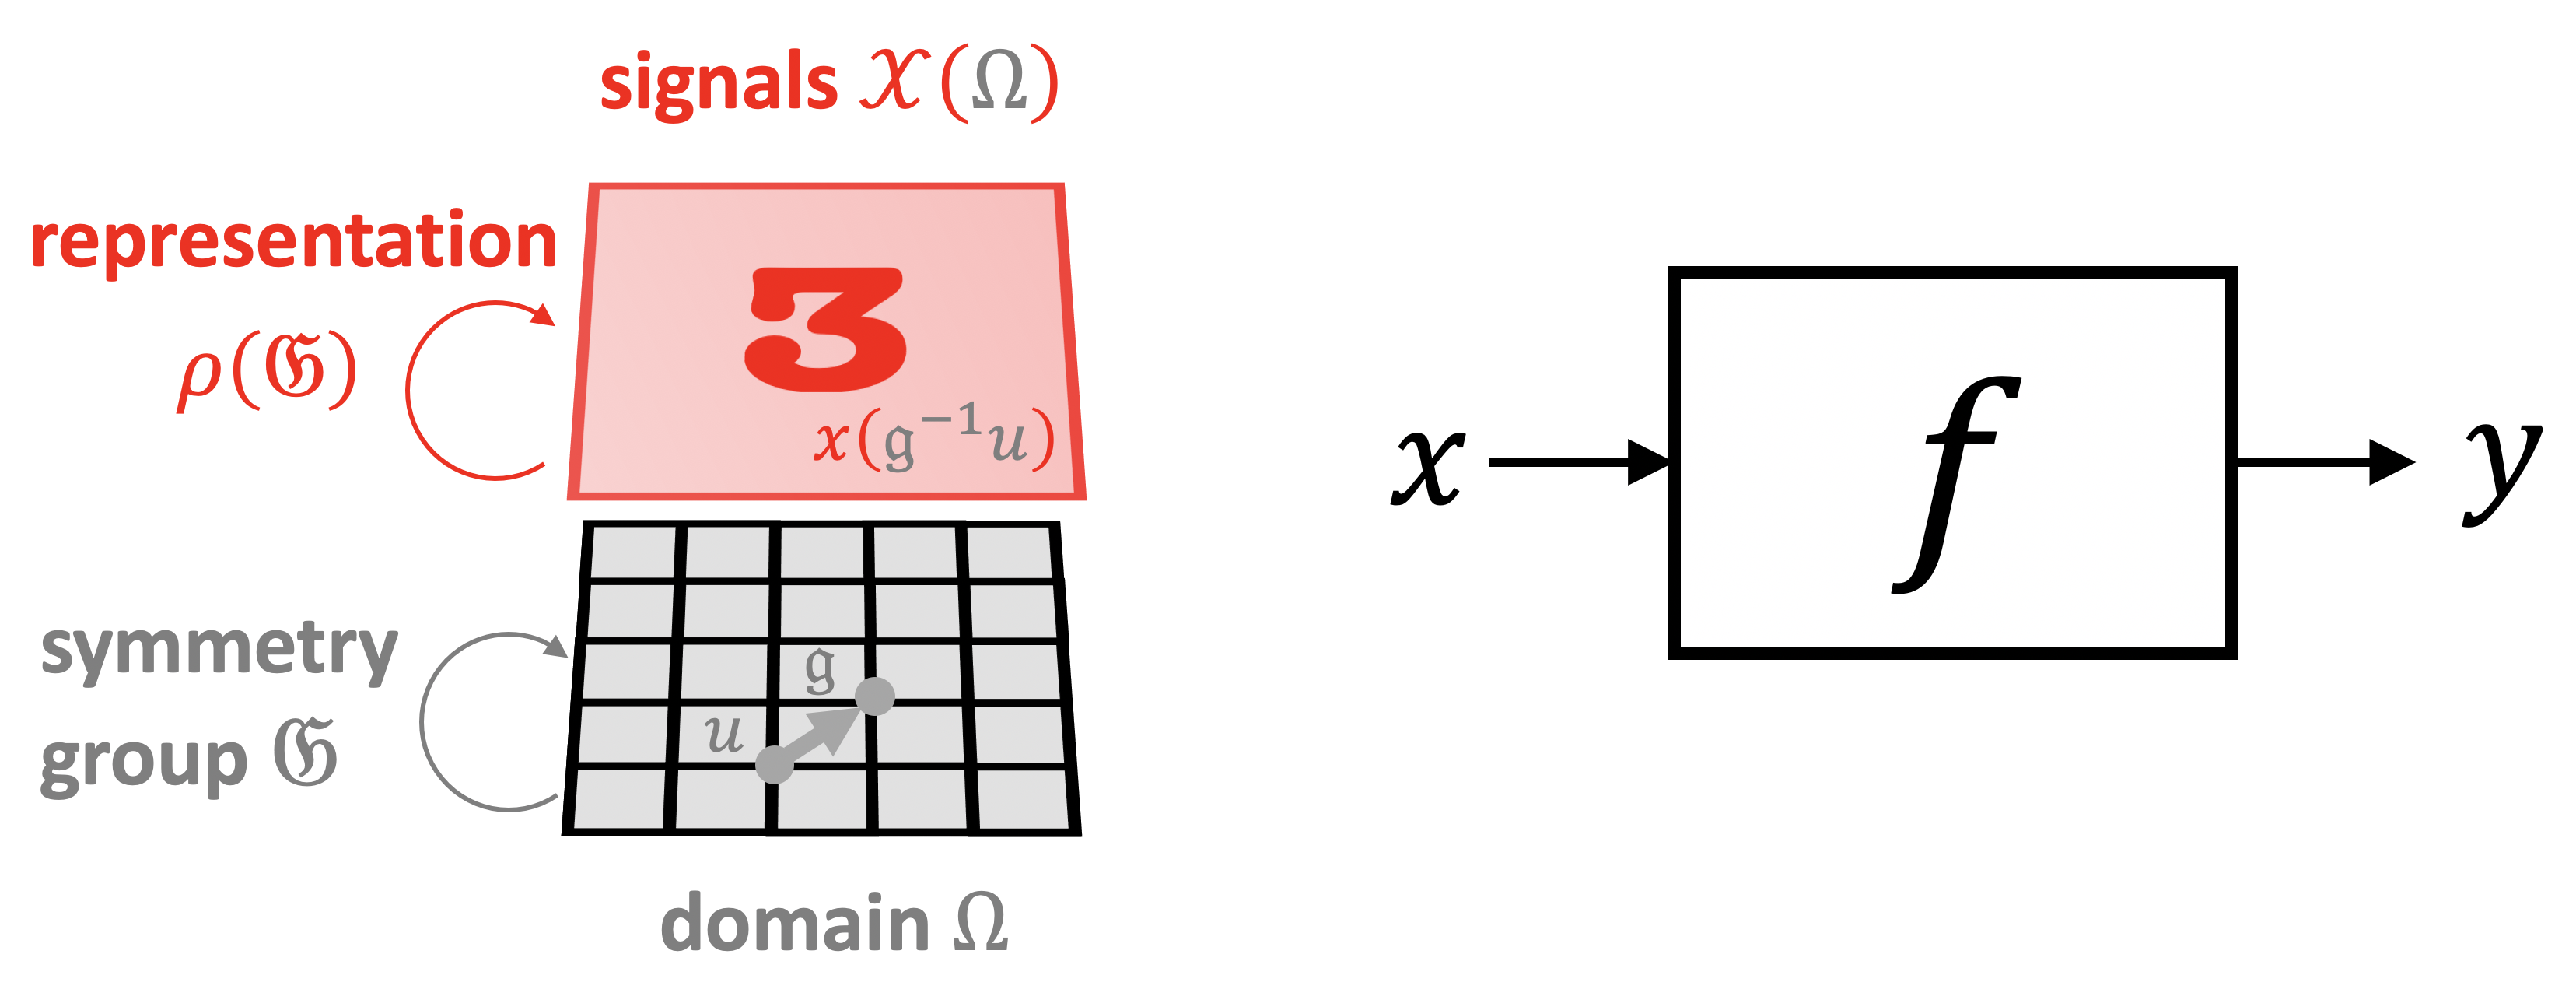
\includegraphics[width=0.75\linewidth]{figures/geom_prior.png}%groups1.pdf}
    \caption{
    几何深度学习所关注的三个空间：（物理）{\em 域} $\Omega$、{\em 信号}空间 $\mathcal{X}(\Omega)$，以及{\em 假设}类 $\mathcal{F}(\mathcal{X}(\Omega))$。
    %
    域 $\Omega$ 的对称性（由群 $\fG$ 刻画）作用于信号 $x\in \mathcal{X}(\Omega)$，这一作用由群表示 $\rho(\fg)$ 实现，从而对作用于这类信号的函数 $f\in \mathcal{F}(\mathcal{X}(\Omega))$ 施加结构。
    }
    \label{fig:symmetryactors}
\end{figure}


\paragraph{不变函数与等变函数}

域 $\Omega$ 是信号 $\mathcal{X}(\Omega)$ 的底层域；它所具有的对称性，会对定义在这类信号上的函数 $f$ 施加结构。
%
事实证明，这是一种强有力的归纳偏置；它提高学习\marginnote{一般而言，$f$ 同时依赖于信号和域，即 $\mathcal{F}(\mathcal{X}(\Omega), \Omega)$。为简洁起见，我们通常省略后一种依赖。}效率，方式是把可能插值函数的空间 $\mathcal{F}(\mathcal{X}(\Omega))$ 缩减为满足对称性先验的函数。
%
%Adding such known symmetries into the function hypothesis class of a machine learning system is a powerful inductive bias, improving learning efficiency by reducing the space of possible interpolants to those which satisfy the symmetry priors. 
%
本文将研究的两个重要情形是{\em 不变}函数与{\em 等变}函数。


%is its output is unaffected by the action of the group on the argument


\begin{tcolorbox}[width=\linewidth,
                  boxsep=0pt,
                  left=7.5pt,
                  right=7.5pt,
                  top=7.5pt,
                  bottom=7.5pt,
                  arc=0pt,
                  boxrule=0pt,toprule=0pt,
                  colback=boxgray,
                  ]%%
    函数 $f: \mathcal{X}(\Omega) \rightarrow \mathcal{Y}$ 是 $\fG$-{\em 不变的}，如果
    $
    f(\rho(\fg)x) = f(x)$ 对所有 $\fg \in \fG$ 和 $x \in \mathcal{X}(\Omega)$ 都成立；也就是说，其输出不受输入上群作用的影响。
\end{tcolorbox}


不变性的一个经典例子是{\em 平移不变性}，\marginnote{注意，信号处理书籍通常使用“平移不变性”一词来指平移等变性，例如线性平移不变系统。}
它出现在图像分类等计算机视觉与模式识别应用中。此时函数 $f$（通常实现为卷积神经网络）输入一幅图像，并输出该图像包含某个类别对象（例如猫或狗）的概率。%
%
通常可以合理假设，分类结果不应受到对象在图像中位置的影响，即函数 $f$ 必须具有平移不变性。
%
多层感知机虽然能够逼近任何光滑函数，却不具备这一性质；这是二十世纪七十年代将这类架构应用于模式识别问题的早期尝试失败的原因之一。
%
以卷积神经网络为典型代表的局部权重共享神经网络架构，其发展动力之一正是实现平移不变的物体分类。


然而，如果更仔细地考察 CNN 的卷积层，就会发现它们并非平移不变，而是{\em 平移等变的}：换言之，将卷积层的输入平移一定距离，会使输出特征图平移相同距离。

\begin{tcolorbox}[width=\linewidth,
                  boxsep=0pt,
                  left=7.5pt,
                  right=7.5pt,
                  top=7.5pt,
                  bottom=7.5pt,
                  arc=0pt,
                  boxrule=0pt,toprule=0pt,
                  colback=boxgray,
                  ]%%
    函数 $f: \mathcal{X}(\Omega) \rightarrow \mathcal{X}(\Omega)$ 是 $\fG$-{\em 等变的}，如果\marginnote{
    更一般地，可能有 $f: \mathcal{X}(\Omega) \rightarrow \mathcal{X}(\Omega')$，其中输入与输出空间具有不同的域 $\Omega, \Omega'$ 和表示 $\rho$、$\rho'$，而这些表示属于同一个群 $\fG$。
    在这种情况下，等变性定义为 $f(\rho(\fg)x) = \rho'(\fg) f(x)$。
    %symmetry groups, $\fG$ and $\fG'$. In this case, equivariance is defined as $ f(\rho(\fg)x) = \rho'(\fg) f(x)$, where $\rho'$ is the representation of $\fG'$.
    } 
    $f(\rho(\fg)x) = \rho(\fg) f(x)$ 对所有 $\fg \in \fG$ 都成立；也就是说，输入上的群作用以相同方式影响输出。
\end{tcolorbox}




再次以计算机视觉为例，需要平移等变性的典型应用是图像分割，其中 $f$ 的输出是逐像素图像掩码。
%
显然，分割掩码必须随输入图像的平移而移动。
在本例中，输入域与输出域相同；但由于输入有三个颜色通道，而输出对每个类别有一个通道，因此表示 $(\rho, \mathcal{X}(\Omega, \mathcal{C}))$ 与 $(\rho', \mathcal{X}(\Omega, \mathcal{C}'))$ 略有不同。


不过，即使是前述图像分类用例，通常也是由一系列卷积（平移等变）层实现，随后接全局池化（平移不变）。
%
正如第~\ref{sec:gdl_blueprint} 节将看到的，这是包括 CNN 和图神经网络（GNN）在内的大多数深度学习架构的一般蓝图。
%: a sequence of equivariant layers, optionally followed by invariant layers. 


%In supervised learning, the goal is to approximate some function $f : \mathcal{X} \rightarrow \mathcal{X}'$ from a finite set of samples.
%In many cases, the problem has symmetries, which means that $f$ is either invariant ($f(\rho(\fg) x) = f(x)$ for all $\fg \in \fG$) or equivariant ($f(\rho(\fg) x) = \rho'(\fg) f(x)$).
%For instance, in image classification the class label is invariant, whereas the segmentation mask is equivariant. 
% In machine learning, where one tries to approximate some unknown function $f$ from a finite set of samples, $f$ often has known symmetries.
% Canonical examples include translations in computer vision and image classification tasks, rotations in molecular prediction problems, or permutations in 3D graphics point-cloud processing tasks. 
% %
% In such settings, given some domain $\gX$ with a certain symmetry group $\fG$, we say that 
% $f: \gX \to \gY$ is $\fG$\emph{-invariant} if $f(\fg.x) = f(x)$ for all $x\in \gX$ and $\fg \in \fG$. If in addition $\fG$ is also acting on $\gY$, we say that $f$ is $\fG$\emph{-equivariant} if $f(\fg.x) = \fg.(f(x))$.
% % We will explore these concepts in detail in Chapter ??. 
%Adding such known symmetries into the function hypothesis class %$\gF$ 
%of a machine learning system is a powerful inductive bias, improving learning efficiency by reducing the space of possible interpolants to those which satisfy the symmetry priors. 


% Possible todo's for this section:
% Explain in/equivariance mathematically (at a high level only)
% Explain group representations (idem)


%\taco{TODO: add definition of space of signals, and regular rep acting on it}

%\taco{TODO: Figure showing domain Omega, group action of G on Omega, and the space of functions X on Omega}

\subsection{同构与自同构}
\label{sec:isomorphism}

\paragraph{子群与结构层次}

如前所述，对称性\marginnote{不同对象之间保持结构的可逆映射通常统称为{\em 同构}（希腊语意为“形状相同”）。对象到自身的同构称为{\em 自同构}，即对称性。}
%We will mainly use this term for maps preserving the connectivity of graphs.}
是保持某种性质或结构的变换；对于给定结构，所有这类变换的集合构成一个对称群。
我们关注的结构往往不止一种，因此可以在域 $\Omega$ 上考虑若干{\em 结构层次}。
%
%We can thus formalise symmetries as invertible maps $\tau: \Omega \rightarrow \Omega$ that preserve some structure. % and satisfy the group axioms with the function composition operation.  
因此，何种变换算作对称性取决于所考虑的结构；但在所有情况下，对称性都是尊重该结构的可逆映射。

在最基本的层次上，域 $\Omega$ 是一个\emph{集合}，所含结构最少：只能说该集合具有某个\emph{基数}\marginnote{对于有限集，基数是集合中的元素数量（“大小”）；对于无限集，基数表示不同类型的无穷，例如自然数的可数无穷，或连续统 $\R$ 的不可数无穷。}。%, and which elements are members of the set.
保持这种结构的自映射是\emph{双射}（可逆映射），可以将其视为集合层次的对称性。
%A more formal way to say the same is that the automorphism group $\mathrm{Aut}(\Omega)$ in the category of sets is the group of bijections $\tau : \Omega \rightarrow \Omega$.
%Such maps are often referred to as (set-){\em automorphisms} and denoted by $\mathrm{Aut}(\Omega)$. 
%
通过检查公理可以容易地验证这构成一个群：两个双射的复合仍是双射（封闭性）；结合律来自函数复合的结合律；映射 $\tau(u)=u$ 是单位元；并且按定义，每个 $\tau$ 都存在逆，满足 $(\tau \circ \tau^{-1})(u) = (\tau^{-1} \circ \tau)(u) =u$。


根据具体应用，还可能存在更高的结构层次。
%
例如，如果 $\Omega$ 是拓扑空间，可以考虑保持{\em 连续性}的映射：这类映射称为{\em 同胚}；除去集合之间双射这一要求外，它们自身连续，逆映射也连续。
%
直观地说，连续函数具有良好性质，它把点 $u$ 周围某邻域（开集）中的点映射到 $\tau(u)$ 周围的一个邻域中。
%Thus, homeomorphisms $\tau : \Omega \rightarrow \Omega$ are the automorphisms / symmetries of $\Omega$ viewed as a topological space.


%
%
还可以进一步要求映射及其逆都是（连续）{\em 可微的}，\marginnote{每个可微函数都是连续的。如果映射“足够多次”连续可微，则称其为{\em 光滑的}。}即映射及其逆在每一点都有导数（且导数也连续）。
%
这需要可微流形所具有的进一步可微结构；在这种结构下，这类映射称为{\em 微分同胚}，记为 $\mathrm{Diff}(\Omega)$。
%These are the automorphisms of smooth manifolds.
%
%
后文还会遇到其他结构，例如{\em 距离}或{\em 度量}（保持它们的映射称为{\em 等距变换}），以及{\em 取向}（据我们所知，保持取向的映射没有通用的希腊语名称）。


\begin{tcolorbox}[width=\linewidth,
                  boxsep=0pt,
                  left=7.5pt,
                  right=7.5pt,
                  top=7.5pt,
                  bottom=7.5pt,
                  arc=0pt,
                  boxrule=0pt,toprule=0pt,
                  colback=boxgray,
                  ]%%
{\em 度量}或{\em 距离}是函数 $d:\Omega\times\Omega \rightarrow [0,\infty)$，并对所有 $u,v,w \in \Omega$ 满足：\vspace{3mm}\\
%\begin{enumerate}
    %\item 
    \noindent {\em 	同一性：} $d(u,v) =0$ 当且仅当 $u=v$。\vspace{2mm}\\
    \noindent  {\em 对称性：} $d(u,v) = d(v,u)$。\vspace{2mm}\\
    \noindent  {\em 三角不等式：} $d(u,v) \leq  d(u,w) + d(w,v)$。\vspace{2mm}\\
%\end{enumerate}

配备度量的空间 $(\Omega,d)$ 称为{\em 度量空间}。

\end{tcolorbox}




%an image plane can be viewed as a smooth manifold, in which case any smooth deformation (diffeomorphism) should be considered a symmetry.
%In practice the object identity will not be preserved by arbitrarily large deformations, so we may add a distance metric, i.e. view the image plane as a Riemannian manifold, in which case only distance-preserving transformations (isometries) can be considered as symmetries.
%As a further example, independently of whether we care about distances, we can assign an \emph{orientation} to the plane, i.e. clockwise or counterclockwise, and consider only orientation-preserving transformations.

应当考虑何种结构层次取决于具体问题。
例如，在分割组织病理学切片图像时，我们可能希望把图像的翻转版本视为等价（因为样本放到显微镜下时可以翻转）；但在对道路标志分类时，则只希望把保持取向的变换视为对称性（因为反射可能改变标志的含义）。
%{\bf [Figure?]}

随着需要保持的结构层次增加，对称群会变小。
事实上，增加结构等价于选择一个\emph{子群}；子群是较大群的一个子集，其自身满足群公理：
%(i.e. it is closed under composition and inverses, and contains the identity).
 
 \begin{tcolorbox}[width=\linewidth,
                   boxsep=0pt,
                   left=7.5pt,
                   right=7.5pt,
                   top=7.5pt,
                   bottom=7.5pt,
                   arc=0pt,
                   boxrule=0pt,toprule=0pt,
                   colback=boxgray,
                   ]%%
 设 $(\fG,\circ)$ 为一个群，$\mathfrak{H} \subseteq \fG$ 为一个子集。称 $\mathfrak{H}$ 是 $\fG$ 的{\em 子群}，如果 $(\mathfrak{H},\circ)$ 在同一运算下构成群。
 \end{tcolorbox}
 
例如，欧氏等距变换群 $\E{2}$ 是平面微分同胚群 $\diff{2}$ 的子群，而保持取向的等距变换群 $\SE{2}$ 又是 $\E{2}$ 的子群。
这一结构层次遵循前言所述的 Erlangen Programme 思想：在 Klein 的构造中，射影几何、仿射几何与欧氏几何具有逐渐增多的不变量，并对应于逐渐缩小的群。


\paragraph{同构与自同构}
% Optional: discuss the notion of isomorphic objects, and present symmetries as self-isomorphisms i.e. automorphisms. Thus the notion of symmetry depends on the notion of iso, i.e. the category we're working in, i.e. the level of structure as discussed above.

我们已经把对称性描述为\emph{从对象到其自身}的、保持结构的可逆映射。
这类映射也称为\emph{自同构}，描述对象与其自身等价的一种方式。
然而，还有一类同样重要的映射称为\emph{同构}，用于表明两个不同对象之间的等价性。
这些概念经常被混淆，但为了使后续讨论清晰，有必要将其区分开来。

为理解二者的区别，考虑集合 $\Omega = \{0,1,2\}$。
集合 $\Omega$ 的自同构是双射 $\tau : \Omega \rightarrow \Omega$，例如循环移位 $\tau(u) = u + 1 \mod 3$。
这种映射保持基数性质，并把 $\Omega$ 映射到自身。
如果另有一个元素数量相同的集合 $\Omega' = \{a, b, c\}$，那么双射 $\eta : \Omega \rightarrow \Omega'$，例如 $\eta(0) = a$、$\eta(1) = b$、$\eta(2) = c$，就是一个{\em 集合同构}。

正如第~\ref{sec:proto-graphs} 节将针对图说明的，%$\Omega$,
结构的概念不仅包括节点数量，也包括连通性。
因此，同构 $\eta: \mathcal{V} \rightarrow \mathcal{V}'$ 位于两个图 $\mathcal{G}=(\mathcal{V},\mathcal{E})$ 与 $\mathcal{G}'=(\mathcal{V}',\mathcal{E}')$ 之间，是节点之间的双射；它把相连节点对映射为相连节点对，也把不相连节点对映射为不相连节点对。\marginnote{即 $(\eta(u),\eta(v)) \in \mathcal{V}'$ 当且仅当 $(u,v) \in \mathcal{V}$。}因此，两个同构图在结构上完全相同，区别仅在于节点次序。\marginnote{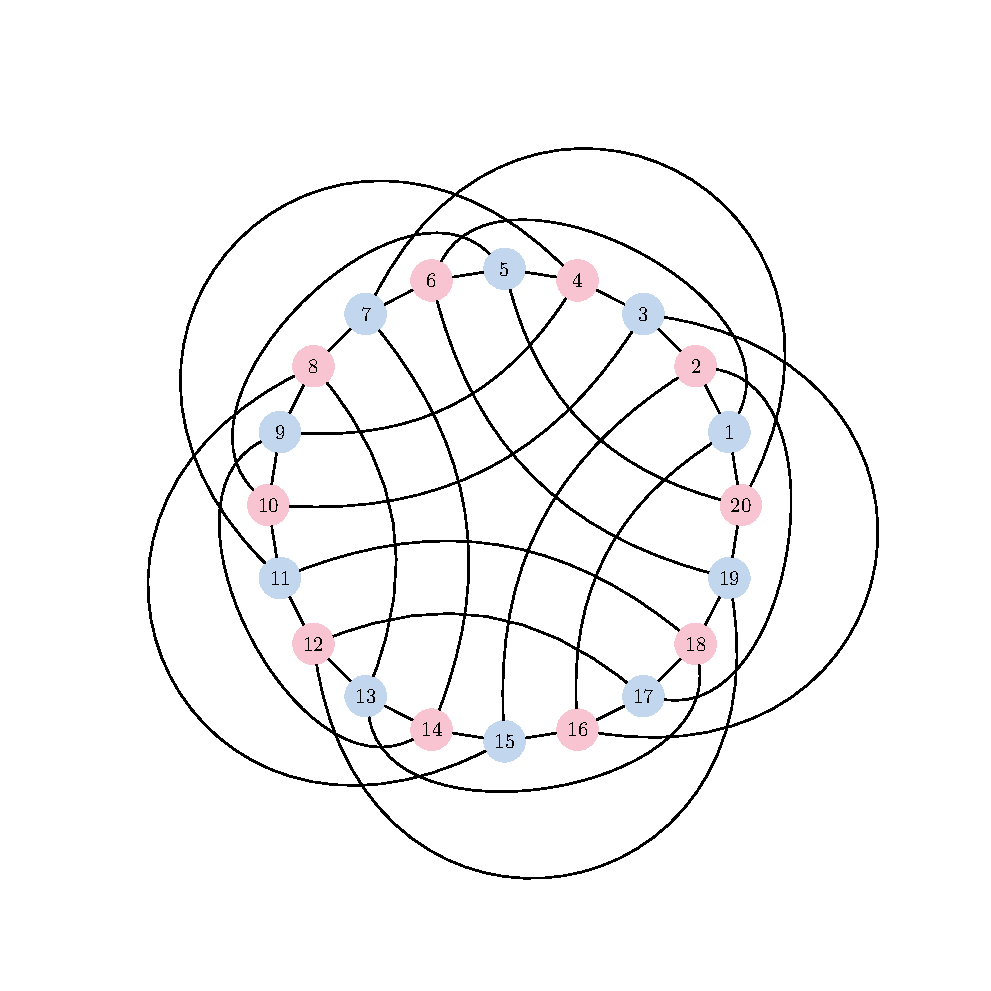
\includegraphics[width=\linewidth]{figures/folkman_g.pdf}\vspace{-2mm}\\ \emph{Folkman graph} \citep{folkman1967regular} 是一个具有 3840 个自同构的优美图实例，这一点可由绘制它的多种对称方式体现。}
%
另一方面，图的自同构或对称性是映射 $\tau : \mathcal{V} \rightarrow \mathcal{V}$；它在保持连通性的同时，把图的节点映射回自身。具有非平凡自同构（即 $\tau \neq \mathrm{id}$）的图呈现出对称性。
%\michael{Show in a figure}

%An isomorphism of graphs is thus not the same as a symmetry, but it is just as important that our neural network treat isomorphic objects equivalently.
% when we're dealing with isos vs autos. Example of sphere and graph

% same number of isos A -> B and autos A -> A. Isomorphic objects have isomorphic automorphism groups




\subsection{形变稳定性}
\label{sec:geom_stab}
%While the Fourier representation is useful to represent {\em signals} $\gX(\Omega)$ on a domain $\Omega$, it is not necessarily useful to regularise the space of {\em functions on such signals}, $\mathcal{F}(\mathcal{X}(\Omega))$ used in supervised learning problems. 
%
%Despite its far-reaching implications, the Fourier representation $\hat{x}$ is not necessarily useful to regularise the space of functions $\{ f : \gX \to \gY \}$, 
%the ultimate goal of supervised learning. 
%
第~\ref{sec:symmetries}--\ref{sec:isomorphism} 节引入的对称性形式体系刻画了一个理想化世界：我们确切知道哪些变换应被视为对称性，并希望{\em 精确地}尊重这些对称性。
%the transformations affecting the input are captured with simple mathematical models.
例如，在计算机视觉中，可以假设平面平移是精确对称性。
%model for input variability parametrised by only two degrees of freedom (the translations in the plane). 
然而，现实世界含有噪声，这种模型在两个方面存在不足。%: it only describes \emph{global} transformations, and

\marginnote{
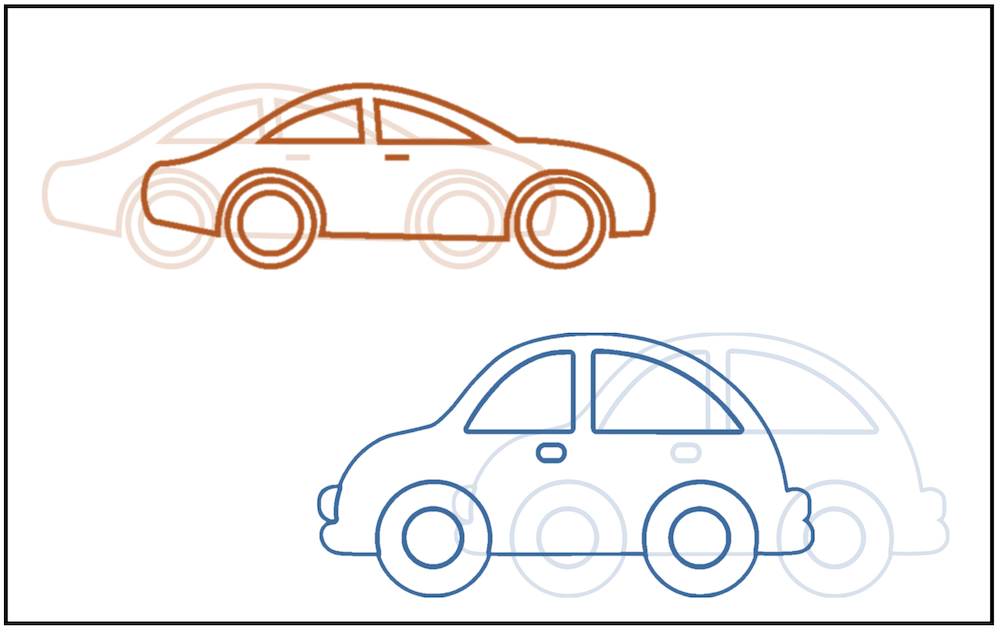
\includegraphics[width=0.95\linewidth]{figures/videosketch.png}
视频中以不同速度运动的两个对象定义了
平移群之外的变换。
}
首先，尽管这些简单群提供了理解域 $\Omega$ 的\emph{全局}对称性（进而理解其上信号 $\gX(\Omega)$ 的全局对称性）的方法，却不能很好地刻画\emph{局部}对称性。
%
例如，考虑一个视频场景%$x=x_t$
，其中有若干对象，每个对象都沿各自不同的方向运动。
在后续帧中，所得场景
%$x_{t+\delta t}$ 
将包含近似相同的语义信息，但没有任何全局平移能够解释一帧到另一帧的变换。
在其他情况下，例如摄像机观察到的可形变三维对象，要描述保持对象身份的变换群本身就非常困难。
这些例子说明，在现实中，我们更关心一个%beneath the global symmetry group lies a
大得多的变换集合，其中全局的精确不变性被局部的非精确不变性所取代。
%
在讨论中，我们将区分两种情形：一种是域 $\Omega$ 固定而信号 $x \in \gX(\Omega)$ 经历形变；另一种是域 $\Omega$ 本身可能发生形变。
%\taco{TODO: perhaps move this up, and discuss this as isomorphisms vs automorphisms?}

%In the language of group representations, we thus need to account for a broader class of bijective domain transformations called {\em automorphisms}, $\mathrm{Aut}(\Omega) = \{ \tau: \Omega \xrightarrow{1:1} \Omega \}$. 
\paragraph{对信号形变的稳定性}
在许多应用中，我们先验地知道，信号 $x$ 的小形变不应改变 $f(x)$ 的输出，因此很自然地会想把这类形变视为对称性。
例如，可以把小微分同胚 $\tau \in \diff{\Omega}$，甚至小双射，视为对称性。
然而，小形变可以复合成大形变，因此“小形变”不构成群\marginnote{例如，两个 $\epsilon$-等距变换的复合是一个 $2\epsilon$-等距变换，违反封闭性。}，也就不能只要求对小形变具有不变性或等变性。
由于大形变确实可能实质性改变输入的语义内容，因此把完整群 $\diff{\Omega}$ 用作对称群也并不可取。

更好的方法是，量化给定的 $\tau \in \diff{\Omega}$ 距给定对称子群 $\fG \subset \diff{\Omega}$（例如平移）有多“远”，所使用的复杂度度量为 $c(\tau)$，
并要求 $c(\tau) = 0$；每当 $\tau \in \fG$ 时，这一等式都成立。
这样，便可以用一种更“柔和”的\emph{形变稳定性}（或{\em 近似不变性}）概念，取代之前关于群作用下精确不变性与等变性的定义：
\begin{equation}
\label{eq:defstability1}
\| f(\rho(\tau) x) - f(x)\| \leq C c(\tau) \|x\|,~,~    \forall x\in \gX(\Omega)
\end{equation}
其中，与前面一样，$\rho(\tau)x(u) = x(\tau^{-1} u)$；$C$ 是与信号 $x$ 无关的某个常数。
满足上述等式的函数 $f\in \mathcal{F}(\mathcal{X}(\Omega))$ 称为{\em 几何稳定的}。
%
下一节~\ref{sec:scale_separation} 将给出这类函数的实例。


由于 $c(\tau)=0$ 对 $\tau \in \fG$ 成立，该定义推广了上文定义的 $\fG$-不变性性质。它在应用中的效用取决于是否引入适当的形变代价。对于定义在连续欧氏平面上的图像，
一种常见选择是 $c^2(\tau) := \int_\Omega \| \nabla \tau(u)\|^2 \mathrm{d}u$，它衡量 $\tau$ 的“弹性”，即它与常向量场位移之间的差异程度。
%
这种形变代价实际上是一个范数，通常称为{\em Dirichlet 能量}，可用于量化 $\tau$ 距平移群有多远。

%


% All of the symmetry groups we have considered and will consider in this book are subgroups of the group of bijections of $\Omega$.
% %The symmetry groups we have considered so far are subgroups of the group $\mathrm{Aut}(\Omega)$ of set-automorphisms of $\Omega$, or general domain transformations. 
% %
% For any such group $\fG$, 

% Same way as we had the symmetry group $\fG$ represented as a linear operator $\rho$ on $\mathcal{X}(\Omega)$, we can now do the same for $\mathrm{Aut}(\Omega)$ to lift diffeomorphisms of the domain into linear transformations on signals $x \in \gX(\Omega)$:
% %construct a linear operator $L_\tau: \gX(\Omega) \to \gX(\Omega)$ of the form 
% %that extend group actions, and which again lift into linear transformations , 
% $$
% (\rho(\tau) x)(u) = x( \tau^{-1}(u)). 
% $$  
% %$\rho(\fg), \fg \in \fG$, we thus need to consider linear transformations
% %
% This represents how the transformation of the domain $\Omega$ by an automorphism $\tau$ affects the signal $x \in \mathcal{X}(\Omega)$; see Figure \ref{fig:groupdeformation}. %
% Note that invariance to such large automorphism group is not a desired property, since large distortions of the domain 
% eventually destroy the semantic information of the input. 
% Instead, we can quantify how "far" a given $\tau \in \mathrm{Aut}(\Omega)$ is from a given symmetry subgroup $\fG \subset \mathrm{Aut}(\Omega)$ 
% with a complexity measure $c(\tau)$, so that $c(\tau) = 0$ whenever $\tau \in \fG$. 
% We can now replace our previous rigid definition of invariance and equivarance under group actions to a softer 
% \emph{deformation stability} principle:
% %Similarly to our definition of functions that are invariant and equivariant under group actions, 
% %we can have functions that are {\em approximately invariant} or {\em equivariant} under such automorphisms. 
% %
% %Such approximate invariance, to which we refer as {\em geometric stability}, can be expressed in the form of a bound %of the form
% \begin{equation}
% \label{eq:defstability1}
% \forall ~x\in \gX(\Omega)~,~\| f(\rho(\tau) x) - f(x)\| \leq C c(\tau) \|x\|,    
% \end{equation}
% with some constant $C$ independent of the signal $x$. A function $f\in \mathcal{F}(\mathcal{X}(\Omega))$ satisfying the above equation is said to be {\em geometrically stable}. 
% %
% Since $c(\tau)=0$ for $\tau \in \fG$, this definition generalises the $\fG$-invariance property defined above. Its utility in applications depends on introducing an appropriate deformation cost. In the case of images defined over a continuous Euclidean plane, 
% a relevant example is given by $c^2(\tau) := \int_\Omega \| \nabla \tau(u)\|^2 \mathrm{d}u$. This deformation cost is in fact a norm often called the {\em Dirichlet energy}, and used as a measure of elasticity of $\tau$. 
% %We will discuss these concepts in greater detail in Chapter ???.

% %To quantify this properly, we need some notion of metric or `distance' between maps and signals, as will be detailed in Section ??.  
% %
% %In some sense that will be formalized later, we expect our functions of interest to be \emph{almost} invariant/equivariant for transformations $L_\tau$ which are ``nearby" the group transformations $\rho(\fg)$ for $\fg \in \fG$.
% %We informally refer to this concept as \emph{geometric stability}. 

\begin{figure}[!htbp]
    \centering
    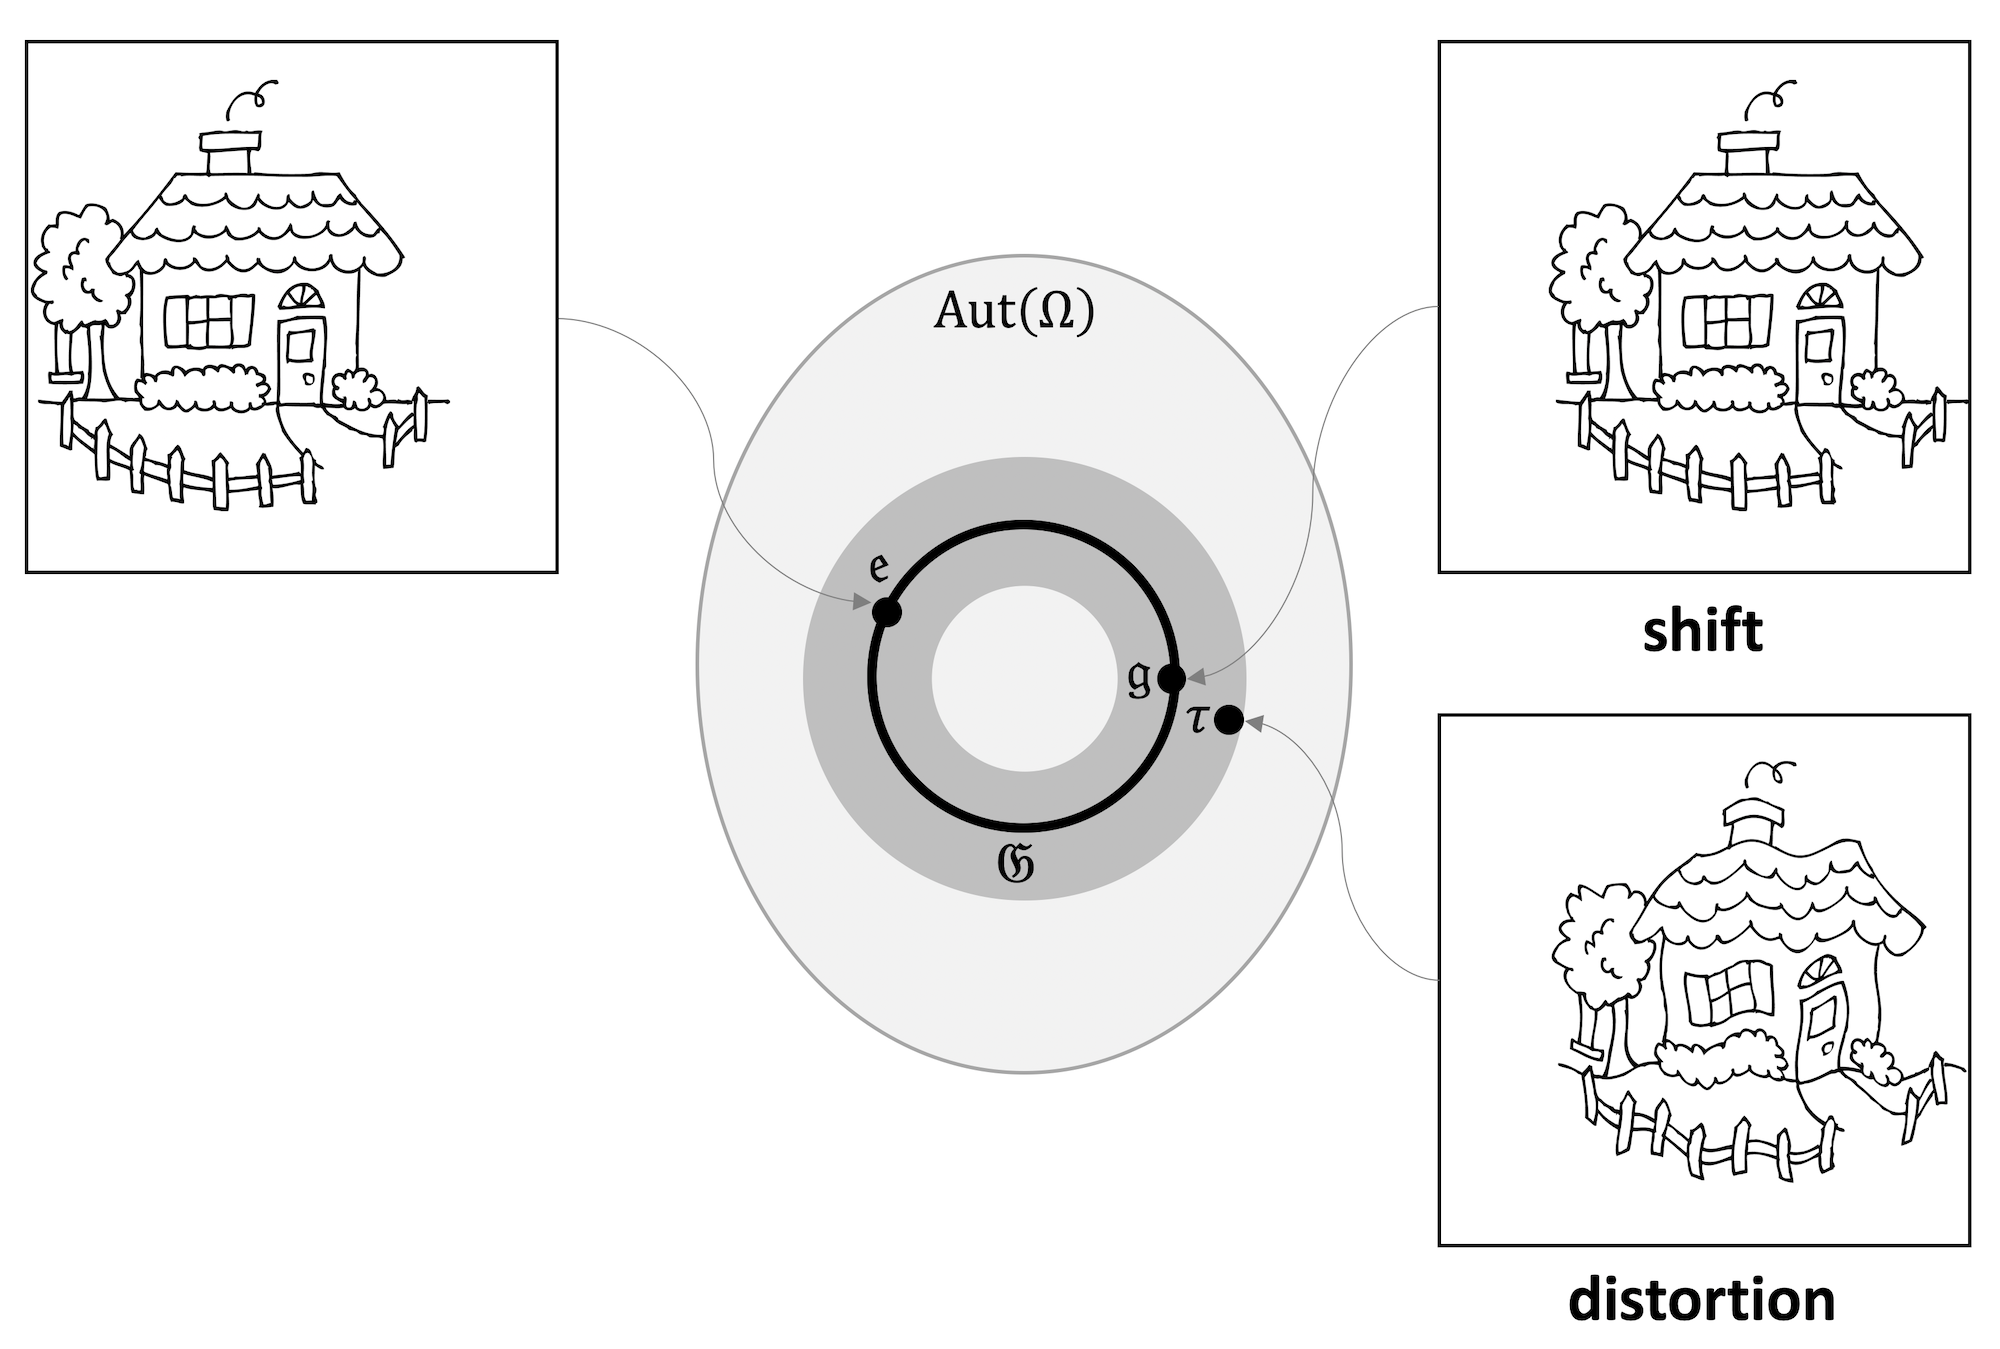
\includegraphics[width=1\textwidth]{figures/g_autg.png}
    \caption{从 $\Omega$ 到其自身的所有双射构成\emph{集自同构群} $\mathrm{Aut}(\Omega)$，对称群 $\fG$（图中圆形）是它的子群。几何稳定性把 $\fG$-不变性与等变性的概念推广到“$\fG$ 周围的变换”（图中灰色圆环）；这种邻近关系由变换之间的某种度量来量化。
    在本例中，图像的光滑畸变接近一次平移。
    }
    \label{fig:groupdeformation}
\end{figure}

%\begin{figure}
%    \centering
%    \includegraphics[width=0.7\textwidth]{figures/deform_image.pdf} \\
%    \includegraphics[width=0.7\textwidth]{figures/shapedef.pdf} \\
%        \includegraphics[width=0.4\textwidth]{figures/protein.jpg}
%    \caption{Examples of Deformations across different domains with a strong 
%    geometric stability prior. \michael{Better show a small molecule with a rotamer? Perhaps show just two examples of each?} }
%    \label{fig:deformation}
%\end{figure}

\paragraph{对域形变的稳定性}
在许多应用中，发生形变的对象不是信号，而是几何域 $\Omega$ 本身。处理图和流形的应用是典型实例：图可以对不同时刻、包含略有不同社会关系（关注图）的社交网络建模；流形则可以对经历非刚性形变的三维对象建模。
%The intuition that one can slightly bend or twist a manifold can be formalized by considering a 
这种形变可以按如下方式量化。若 $\mathcal{D}$ 表示所有可能的可变域空间（例如所有图的空间或 Riemann 流形空间），则可以对 $\Omega, \tilde{\Omega} \in \mathcal{D}$ 定义适当的度量（“距离”）$d(\Omega, \tilde{\Omega})$，并要求 $d(\Omega,\tilde{\Omega})=0$ 在 $\Omega$ 与 $\tilde{\Omega}$ 于某种意义下等价时成立。例如，当两个图同构时，图编辑距离为零；当两个配备测地距离的 Riemann 流形等距时，它们之间的 Gromov-Hausdorff 距离为零。\marginnote{图编辑距离衡量通过一系列图编辑操作使两个图同构所需的最小代价。Gromov-Hausdorff 距离衡量两个度量空间之间某种对应关系可能达到的最小度量畸变；见 \cite{gromov1981structures}。}


构造这类域间距离的一种常见方法依赖于某个可逆映射族
%We assume that this metric comes with an 
$\eta: \Omega \to \tilde{\Omega}$，它试图以尽可能保持相应结构的方式“对齐”这些域。%This can be quantified for, %that is,
例如，对于图或 Riemann 流形（将其视为带测地距离的度量空间），这种对齐可以比较成对的邻接结构或距离结构（分别为 $d$ 和 $\tilde{d}$），%the alignment of graphs
%two graphs with $n$ nodes can be aligned 
%
$$d_{\gD}(\Omega, \tilde{\Omega}) =  \inf_{\eta \in \fG}\|d - \tilde{d}\circ (\eta \times \eta)\|$$
%
%$$d(\Omega, \Omega') = \inf_{\eta \in \fG} %\| e(\Omega) - \eta e(\Omega') \|~,$$
其中 $\fG$ 是由双射或等距变换等同构组成的群，而范数定义在乘积空间 $\Omega \times \Omega$ 上。换言之，通过考虑所有保持内部结构的可能对齐，元素 $\Omega,\tilde{\Omega}$ 之间的距离被“提升”为域本身之间的距离。
%rigid 
%symmetries of the domain 
%(e.g. permutations for graphs, or isometries for Riemannian manifolds), and $e(\cdot)$ is an embedding of the domain (such as the adjacency matrix for a graph, or an Euclidean embedding for a manifold). 
%\michael{Joan: please check. The assumptions on $\eta$ e.g. in GH-metric are very weak, just a bijection}
\marginnote{可以通过二次指派问题（QAP）对齐两个图；在最简单的形式中，它考虑两个图 $G,\tilde{G}$，二者大小相同，均为 $n$，并求解 $\min_{\mathbf{P} \in \Sigma_n} \mathrm{trace}(\mathbf{A P \tilde{A} P}^\top)$，其中 $\mathbf{A}, \tilde{\mathbf{A}}$ 分别为邻接矩阵，$\Sigma_n$ 是 $n \times n$ 置换矩阵群。图编辑距离可以与这类 QAP 联系起来 \citep{bougleux2015quadratic}。
}
给定信号 $x \in \gX(\Omega)$ 和形变后的域 $\tilde{\Omega}$，便可以考虑形变后的信号 $\tilde{x} = x \circ \eta^{-1} \in \gX(\tilde{\Omega})$。
%, $x' := x \circ \varphi^{-1}$.  
%For example, we can define a metri

%metric \emph{in the space of domains}. In other words, two graphs %$G, G'$ can be assigned a distance $d(G,G')$ so that $d(G,G')=0$ iff $G$ and $G'$ are isomorphic, and similarly two Riemannian manifolds $\Omega, \Omega'$ can be compared so that $d(\Omega, \Omega')$ measures the changes in their intrinsic metric structure. 

稍微滥用一下记号，将 $\gX(\mathcal{D}) = \{ (\gX(\Omega), \Omega) \, : \, \Omega \in \mathcal{D} \}$ 定义为在可变域上定义的所有可能输入信号的集合。
如果函数 $f : \gX(\mathcal{D}) \to \gY$ 满足
\begin{equation}
\| f( x, \Omega) - f(\tilde{x}, \tilde{\Omega}) \| \leq C \|x \| d_{\gD}(\Omega, \tilde{\Omega})~
\label{eqn:domain_def_stability}
\end{equation}
%
且该式对所有 $\Omega, \tilde{\Omega} \in \mathcal{D}$ 以及 $x \in \mathcal{X}(\Omega)$ 都成立，则称其对域形变稳定。
%
%\michael{This is not properly defined: we have $x$ defined on both $\Omega$ and $\Omega'$, which requires some notion of correspondence} \joan{added some clarifications}. 
第~\ref{sec:manifolds}--\ref{sec:meshes} 节将在流形语境下讨论这一稳定性概念，其中等距形变起关键作用。
%As we will see in Chapter ??, 
此外，把信号形变稳定性理解为体积形式的形变，可以证明域形变稳定性是信号形变稳定性的自然推广 \cite{gama2019diffusion}。

% %Link between the two via a change of variables. 
% In fact, the two notions of deformation stability are intimately related. Indeed, the deformation operator $L_\tau : \gX \to \gX$ acting on signals can be recast as deforming the inner-product metric, from $\gX = L^2(\Omega, du)$ to $L^2(\Omega,du_\tau)$. In other words, 
% $$\langle L_\tau x, L_\tau y \rangle_{L^2(\Omega), du)} = \int_\Omega x(\tau^{-1}(u)) y(\tau^{-1}(u)) du = \int_\Omega x(u) y(u) |\mathbf{I} - \nabla \tau^{-1}(u) | du := \int_\Omega x(u) y(u) du_\tau~,$$
% so we may view certain signal deformations as specific perturbations of the metric. 

%\michael{Measure not metric? or volume form? I find this section more confusing than helpful, we need to introduce a lot of extra stuff to make it defined properly} \joan{yes, agreed, i simply put a pointer for the future chapter to simplify things for now}. 



\subsection{尺度分离}
\label{sec:scale_separation}

尽管形变稳定性显著增强了全局对称性先验，但它本身仍不足以克服维数灾难；非正式地说，随着域的规模增长，满足式 (\ref{eq:defstability1}) 的函数仍然“太多”。克服这一困难的关键洞见是利用物理任务的多尺度结构。在描述多尺度表示之前，需要先介绍依赖频率而非尺度的 Fourier 变换之主要要素。

\paragraph{Fourier 变换与全局不变量}
可以说，
\marginnote{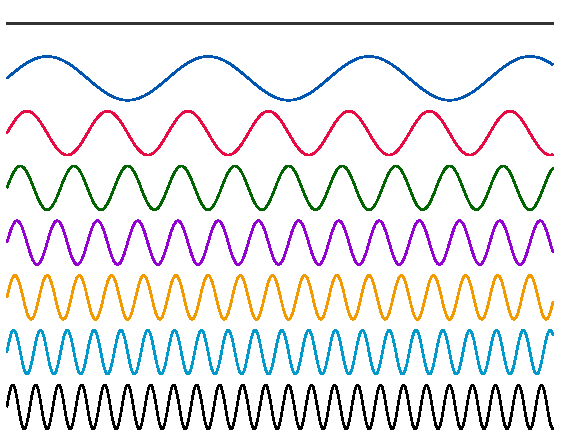
\includegraphics[width=\linewidth]{figures/fourier_basis.pdf}
Fourier 基函数具有全局支撑。因此，局部信号会在所有频率上产生能量。
}
最著名的信号分解是{\em Fourier 变换}，它是调和分析的基石。
%
经典的一维 Fourier 变换
$$
\hat{x}(\xi) = \int_{-\infty}^{+\infty} x(u) e^{-\mi \xi u} \mathrm{d}u
$$
把函数 $x(u) \in L^2(\Omega)$（定义在域 $\Omega = \mathbb{R}$ 上）表示为正交振荡{\em 基函数} $\varphi_\xi(u) = e^{\mi\xi u}$ 的线性组合，
并以它们的振荡速率（或\emph{频率}）$\xi$ 作为索引。按频率组织信号能够揭示其光滑性和局部化等重要信息。
%
%As we will show in Chapter ??, 
Fourier 基本身具有深刻的几何基础，可以解释为域的自然振动，并与域的几何结构相关（例如见 \cite{berger2012panoramic}）。
%\marginnote{Technically, the Fourier transform is defined for functions in $L^2(\Omega) \cup L^1(\Omega)$, and can be extended to a far broader class of generalised functions through the theory of {\em tempered distributions} developed by the Fields laureate Laurent Schwartz. 
%We refer to \cite{mckean} for a wonderful treatment of Fourier Analysis

%

%\begin{figure}
%    \centering
%\includegraphics[width=0.5\linewidth]{figures/fourier1.pdf}
%    \caption{Basic decomposition of a signal into Fourier atoms. Observe that a localized discontinuity in the original signal produces energy across all frequencies.}
%    \label{fig:fourier}
%\end{figure}


%

% \joan{Michael, let me know if you agree. The following paragraph is not strictly needed in this section, and rather belongs to the grid/euclidean domain where we go again through this. I suggest we merge in there.} 
Fourier 变换\marginnote{下文将把卷积与{\em （互）相关}
$$
(x \, \star \,\theta)(u) = \int_{-\infty}^{+\infty} \hspace{-2mm} x(v)\theta(u+v) \mathrm{d}v
$$
互换使用，这在机器学习中十分常见：二者的区别在于滤波器是否反射；由于滤波器通常是可学习的，因此这种区别纯粹只是记号上的。
}在信号处理中起关键作用，因为它给出了{\em 卷积}的对偶表述：
$$
(x\star \theta)(u) = \int_{-\infty}^{+\infty} x(v)\theta(u-v) \mathrm{d}v
$$
这是线性信号滤波的标准模型（这里及下文中，$x$ 表示信号，$\theta$ 表示滤波器）。
%
如下文将说明的，卷积算子在 Fourier 基下被对角化，因此可以把卷积表示为相应 Fourier 变换的乘积：
$$
\widehat{(x\star \theta)}(\xi) = \hat{x}(\xi) \cdot \hat{\theta}(\xi),
$$
这一事实在信号处理中称为卷积定理。
%
%In machine learning, convolution is the cornerstone of Convolutional Neural Networks, an architecture ubiquitously used in computer vision and image analysis applications. 


%Some of the properties of the Fourier transform are intimately related to the geometric properties of the Euclidean space or a grid on which it is defined.    
%The Fourier basis thus diagonalises any convolutional operator. 
事实证明，Laplacian 等许多基本微分算子都可以描述为欧氏域上的卷积。
%, such as the Laplacian $\Delta = \mathrm{div} \, \nabla$. 
由于这类微分算子可以在非常一般的几何上内蕴地定义，因此这提供了一种正式过程，可将 Fourier 变换推广到欧氏域之外，包括图、群和流形。第~\ref{sec:manifolds} 节将对此进行详细讨论。%Chapter~???.

Fourier 变换的一个本质特征是揭示信号与域的\emph{全局}性质，例如光滑性或传导率。当域具有平移等全局对称性时，这种全局行为十分便利，却不适合研究更一般的微分同胚。为此，需要一种能够权衡空间局部化与频率局部化的表示，下面将对此说明。


\paragraph{多尺度表示}
通过
%\marginnote{
%\includegraphics[width=0.9\linewidth]{figures/wavelet.pdf}
%Basic decomposition of a signal into wavelet atoms. Observe that now a localized discontinuity in the original signal creates energy only in the neighborhood of the discontinuity. 
从基于 Fourier 频率的表示切换到{\em 基于尺度的}表示，可以明确表达局部不变性的概念；这种表示是{\em 小波}等多尺度分解方法的基石。\marginnote{全面介绍见 \cite{mallat1999wavelet}。}
%; see Figure \ref{fig:fourier_vs_wavelets} and Insert ??. 
%
多尺度方法的核心洞见，是把定义在域 $\Omega$ 上的函数分解为\emph{在空间和频率上都局部化的}基本函数。\marginnote{
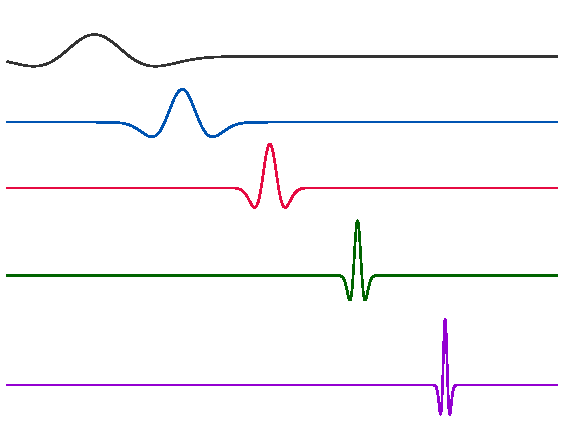
\includegraphics[width=0.9\linewidth]{figures/wavelet_basis.pdf}
%\includegraphics[width=0.9\linewidth]{figures/wavelet.pdf}
与 Fourier 原子不同，小波原子具有局部性和多尺度性，因此可以用空间支撑较小的原子捕获
信号的精细细节，并用空间支撑较大的原子捕获
粗略细节。
%Localized signals create energy only in the neighborhood of the discontinuity. 
这里的\emph{原子}一词与 Fourier 分析中的“基元素”同义，但需要注意，小波是冗余的（过完备的）。
}
对于小波，这是通过与经过平移和伸缩的滤波器（{\em 母小波}）$\psi$ 作相关来实现的，由此产生称为{\em 连续小波变换}的联合时频表示
%
$$
(W_\psi x)(u,\xi) = \xi^{-1/2} \int_{-\infty}^{+\infty} 
\psi\left(\frac{v-u}{\xi}\right) x(v) \mathrm{d}v.
%psi( 2^{j} (u - k2^{-j})) 
%x(u) du \marginnote{In general, $\psi$ can be a complex-valued function, in which case a complex conjugation must be taken in the inner product.}
%(x \star \psi_j)(u)
$$
%
经过平移和伸缩的滤波器称为{\em 小波原子}；% \marginnote{The term \emph{ atom} here is synonymous with `basis element' in Fourier analysis, with the caveat that wavelets are redundant representations that form over-complete bases.}
其空间位置与伸缩分别对应小波变换的坐标 $u$ 和 $\xi$。
%
这些坐标通常按二进方式采样（$\xi=2^{-j}$ 且 $u = 2^{-j}k$），其中 $j$ 称为{\em 尺度}。
%
%
%\int_{-\infty}^{+\infty} 
%\psi( 2^{j} (u - k2^{-j})) 
%x(u) du \marginnote{In general, $\psi$ can be a complex-valued function, in which case a complex conjugation must be taken in the inner product.}
%(x \star \psi_j)(u)
%$$
%
多尺度信号表示在捕获超越全局光滑性的正则性性质（例如分片光滑性）方面具有重要优势，这使其在二十世纪九十年代成为信号与图像处理以及数值分析中的常用工具。

\paragraph{多尺度表示的形变稳定性：}
当考虑底层对称群“附近”的小形变所产生的影响时，多尺度局部化小波分解相对于 Fourier 分解的优势便显现出来。下面在欧氏域和平移群中说明这一重要概念。
由于 Fourier 表示对角化了移位算子（正如第~\ref{sec:grids_euclidean} 节将更详细说明的，该算子可以视为卷积），因此它是平移变换的高效表示。然而，Fourier 分解在高频形变下并不稳定。
%
相比之下，小波分解在这类情形中提供了稳定表示。

事实上，考虑 $\tau \in \mathrm{Aut}(\Omega)$ 及其相关线性表示 $\rho(\tau)$。当 $\tau(u) = u - v$ 是一次平移时，
正如第 \ref{sec:grids_euclidean} 节将验证的，算子 $\rho(\tau) = S_v$ 是与卷积可交换的{\em 移位算子}。
%any convolution operator $H$ of the form $H x = x \star h$, with arbitrary filter $h$. 
由于卷积算子由 Fourier 变换对角化，频域中的平移作用等价于移动 Fourier 变换的复相位：
%
%As a result, by expressing this commutation relationship in the Fourier domain, we have that 
$$
(\widehat{S_v x})(\xi) = e^{-\mi \xi v} \hat{x}(\xi). 
$$ 
%for any frequency $\xi$. 
%Rigid translations are thus expressed in the Fourier domain by simply shifting the (complex) phase of every fourier coefficient of the signal, leading 
因此，去除复相位的{\em Fourier 模} $f(x) = |\hat{x}|$ 是一个简单的平移不变函数，即 $f(S_v x) = f(x)$。
%to simple translation invariant representations by removing this complex phase: $Mx = |\hat{x}|$. In other words, for rigid translations, the Fourier modulus is translation invariant: $\| M - M L_\tau \| = 0$. 
%
然而，如果只有近似平移，
%$\tau(u) \approx u - v$, 
$\tau(u) = u - \tilde{\tau}(u)$ 且 $\|\nabla \tau \|_\infty = \sup_{u\in \Omega} \| \nabla \tilde{\tau}(u)\| \leq \epsilon$，
情况便完全不同：可以证明
$$
\frac{\|f(\rho(\tau) x) - f(x) \| }{ \|x\| }= \mathcal{O}(1)
$$ 
无论 $\epsilon$ 多小（即 $\tau$ 多么接近一次平移），上述结论都成立。因此，这种 Fourier 表示在形变下{\em 不稳定}，无论形变多小。这种不稳定性也出现在一般域和非刚性变换中；第 \ref{sec:geomanifoldsec} 节将使用 Fourier 变换的自然推广分析三维形状，并看到另一个不稳定性实例。

小波为这一问题提供了补救方法，也揭示了多尺度表示的力量。在上述例子中，可以证明 \citep{mallat2012group} 小波分解 $W_\psi x$ 对形变{\em 近似等变}：
$$
\frac{\| \rho(\tau) (W_\psi x) - W_\psi (\rho(\tau) x) \|}{\|x\|} = \mathcal{O}(\epsilon).
\marginnote{This notation implies that $\rho(\tau)$ acts on the spatial coordinate of $(W_\psi x)(u,\xi)$.
}
$$
%and $\gW x = \{ x \star \psi_j \}_j$ is an appropriately normalized wavelet filter bank, then one can verify that wavelet coefficients are nearly \emph{equivariant} to deformations, in the sense that $\| L_\tau \gW - \gW L_\tau \| = O(\epsilon)$. 
%
换言之，使用局部化滤波器而不是频率把信号信息分解到不同尺度，会把全局不稳定表示转化为一族局部稳定特征。重要的是，不同尺度上的这类测量尚不具有不变性，需要逐步向低频处理；这暗示了现代神经网络深层组合的本质，并由下面给出的几何深度学习蓝图加以刻画。


% From our discussion 
% Let us consider a filter $h(u)$ and its associated convolution operator $\gH x = x \star h$. To study how this operator behaves under certain geometric transformations $L_\tau \in \mathrm{Aut}(\Omega)$ we consider the \emph{Lie commutator} 

% Let us consider the Lie commutator $[L_\tau, \gW]= L_\tau \gW - \gW L_\tau$. When $\gW$ is the Fourier transform and $L_\tau$ is exactly a translation, we have $[L_\tau, \gW] = 0$; 
% %Let us denote the decomposition by $U$ and let $L_\tau$ be the deformation operator we have seen before. When $\tau(u) = u-v$ is a pure translation, the Fourier transform satisfies $L_\tau U = U L_\tau$, by virtue of its 
% however when $L_\tau$ is only an approximate translation, then $\| [L_\tau, \gW] \| = O(1)$, irrespective of how close $L_\tau$ is to being a translation. 
% On the other hand, if $\tau(u) = u - \tilde{\tau}(u)$, with $\sup_u \| \nabla \tilde{\tau}(u)\| \leq \epsilon$ (thus $\tau$ is nearly a translation), then one can show \cite{scatt} that when $\gW$ is the overcomplete wavelet transform, $\| [ L_\tau, \gW ] \| \simeq \epsilon$. 





%\paragraph{Scale Separation}
%In our context of high-dimensional learning, multiscale representations such as wavelets serve another fundamental purpose: they provide overcomplete linear decompositions where local translations are nearly equivariant.  
\paragraph{尺度分离先验：}
基于这一洞见，可以考虑把数据域 $\Omega$ 多尺度粗化为层次结构 $\Omega_1, \hdots, \Omega_J$。
%, $j\in [J]$. 
事实证明，这类粗化可以在非常一般的域上定义，包括网格、图和流形。
%capturing a wide range of applications.
非正式地说，粗化把邻近点 $u, u' \in \Omega$ 合并在一起，因此只要求域中具有适当的{\em 度量}概念。
%Geometric objects such as grids, manifolds, Lie groups or Graphs all admit such coarsenings. 
如果 $\gX_{j}(\Omega_j,\mathcal{C}_j) := \{x_j: \Omega_j \to \mathcal{C}_j \}$
%\michael{\bf [MB: why $\R^s$? did not we assume scalar-valued signals for simplicity? ]} 
%\joan{JB: number of channels can vary as we coarsen the domain. But we should keep things simple at this stage, and just describe the general principle without introducing too much notation. } \michael{MB: lets keep it as simple as possible here} 
表示定义在粗化域 $\Omega_j$ 上的信号，那么非正式地说，若函数 $f : \gX(\Omega) \to \gY$ 在尺度 $j$ 上具有形式为 $f \approx f_j \circ P_j $ 的分解，其中 $P_j : \gX(\Omega) \to \gX_{j}(\Omega_j)$ 是非线性\emph{粗粒化}，而 $f_j : \gX_{j}(\Omega_j) \to \gY$，则称该函数在这一尺度上\emph{局部稳定}。换言之，虽然目标函数 $f$ 可能依赖整个域上特征之间复杂的长程交互，但对于局部稳定函数，可以\emph{分离}跨尺度交互：先关注局部化交互，再把它们向较粗尺度传播。

\begin{figure}
    \centering
    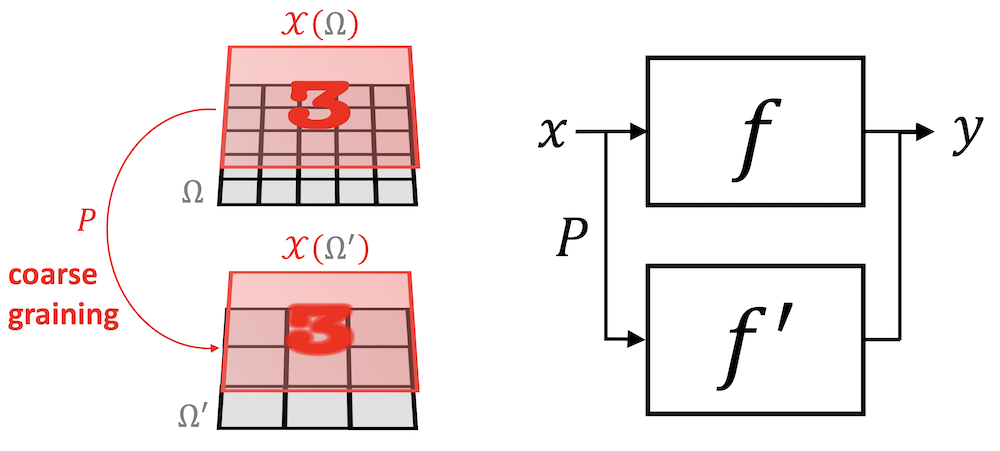
\includegraphics[width=0.75\textwidth]{figures/scale_sep.png}%factorization.pdf}
    \caption{图像分类任务中的尺度分离示意图。分类器 $f'$ 定义在粗网格信号 $\mathcal{X}(\Omega')$ 上，并应满足 $f \approx f'\circ P$，其中 $P: \mathcal{X}(\Omega) \rightarrow \mathcal{X}(\Omega')$。}
    \label{fig:scale_separation}
\end{figure}

这类原则\marginnote{Fast Multipole Method（FMM）是一种数值技术，最初用于加速 $n$ 体问题中长程力的计算。FMM 把彼此接近的源组合起来，并将其视为单一源。
}在物理学与数学的许多领域中具有根本重要性，例如体现在统计物理学所谓的重整化群中，或被 Fast Multipole Method 等重要数值算法利用。在机器学习中，多尺度表示与局部不变性是卷积神经网络和图神经网络高效性的底层基本数学原则，通常以{\em 局部池化}形式实现。在未来工作中，我们将进一步发展计算调和分析工具，在各种几何域上统一这些原则，并阐明尺度分离在统计学习中的优势。





\subsection{几何深度学习蓝图}
\label{sec:gdl_blueprint}

第~\ref{sec:symmetries}--\ref{sec:scale_separation} 节讨论的对称性、几何稳定性与尺度分离原则，可以组合为学习高维数据稳定表示的通用蓝图。
%
这些表示由函数 $f$ 产生；该函数作用于信号 $\mathcal{X}(\Omega,\mathcal{C})$，信号定义在域 $\Omega$ 上，而该域配备对称群 $\fG$。


目前描述的几何先验并未规定构建这类表示的具体{\em 架构}，而是给出了一系列必要条件。
不过，它们暗示了一种公理化构造；可以证明该构造满足这些几何先验，同时保证表示具有很强的表达能力，能够逼近任何满足这类先验的目标函数。%the geometric priors.


一个简单的初步观察是，为得到表达能力很强的表示，必须引入非线性元素，因为
如果 $f$ 是线性的且具有 $\fG$-不变性，那么对所有 $x \in \gX(\Omega)$，\marginnote{这里，$\mu(\fg)$ 称为群 $\fG$ 的\emph{Haar 测度}，积分在整个群上进行。}
$$
f(x) =  \frac{1}{\mu(\fG)} \int_{\fG} f( \fg. x) \mathrm{d}\mu(\fg) = f\left(\frac{1}{\mu(\fG)} \int_{\fG} (\fg.x) \mathrm{d}\mu(\fg) \right),
$$
%\michael{f(x) and not F?}
%\michael{what is $\fg.x$? should be u or use representation $\rho$}
这表明，$F$ 对 $x$ 的依赖仅通过\emph{$\fG$-平均} $A{x} = \frac{1}{\mu(\fG)} \int_{\fG} (\fg.x) \mathrm{d}\mu(\fg)$ 实现。对于图像和平移，这意味着只使用输入的平均 RGB 颜色！%\marginnote{Give a further example for the discrete permutation group, getting the average too}


尽管这一推理表明{\em 线性不变量}族并不丰富，但{\em 线性等变映射}族提供了强大得多的工具，因为通过与适当的非线性映射复合，它能够构造丰富且稳定的特征，下面将对此说明。
%
事实上，若 $B: \gX(\Omega, \gC) \to \gX( \Omega, \gC')$ 具有 $\fG$-等变性，并满足 $B(\fg.x) = \fg.B(x)$，且该式对所有 $x \in \gX$ 和 $\fg \in \fG$ 都成立；再令 $\sigma: \gC' \to \gC''$ 为任意（非线性）映射，则容易验证，复合 $U := (\bm{\sigma} \circ B): \gX(\Omega, \gC) \to \gX( \Omega, \gC'')$ 也具有 $\fG$-等变性。其中，$\bm{\sigma}: \gX(\Omega,\gC') \to \gX(\Omega, \gC'')$ 是 $\sigma$ 的逐元素实例化，定义为 $(\bm{\sigma}(x))(u) := \sigma( x(u))$。

这一简单性质允许定义一个非常一般的 $\fG$-不变量族，方法是把 $U$ 与群平均 $A \circ U : \gX(\Omega, \gC) \to \gC''$ 复合。因此，一个自然问题是：任何 $\fG$-不变函数能否在适当选择 $B$ 和 $\sigma$ 后，由这类模型以任意精度逼近？
%
不难把针对非结构化向量输入的标准通用逼近定理加以调整：通过把群平均适当地推广为一般非线性不变量，可以证明浅层“几何”网络也是通用逼近器。
\marginnote{例如，\citet{zaheer2017deep} 已经为 Deep Sets 模型给出了这类证明。}
%
然而，正如比较 Fourier 不变量与小波不变量时已经说明的，
浅层全局不变性与形变稳定性之间存在根本张力。
这促使我们采用另一种表示，转而考虑\emph{局部化的}等变映射。\marginnote{可以在网格、图、流形和群上定义有意义的度量。一个显著例外是集合，它没有预先定义的度量概念。
%; see Section ? for further discussion.
} 
进一步假设 $\Omega$ 配备距离度量 $d$。若等变映射 $U$ 满足如下条件，则称其为局部化的：$(Ux)(u)$ 只依赖于 $x(v)$ 的值，其中 $\mathcal{N}_u = \{v : d(u,v) \leq r\}$，而 $r$ 是某个较小半径；后一集合 $\mathcal{N}_u$ 称为{\em 感受野}。%$\delta$; .
%\michael{Are we ok to indentify neighbourhood with receptive field?}

单层局部等变映射 $U$ 无法逼近具有长程交互的函数，但多个局部等变映射的复合 $U_J \circ U_{J-1} \dots \circ U_1$ 在保持局部等变映射稳定性性质的同时扩大了感受野\marginnote{“感受野”一词源自神经科学文献，指影响给定神经元输出的空间域。}。通过交错使用粗化域的下采样算子（仍假设具有度量结构），可以进一步扩大感受野，从而完整对应于多分辨率分析（MRA，例如见 \cite{mallat1999wavelet}）。

\begin{figure}
    \centering
    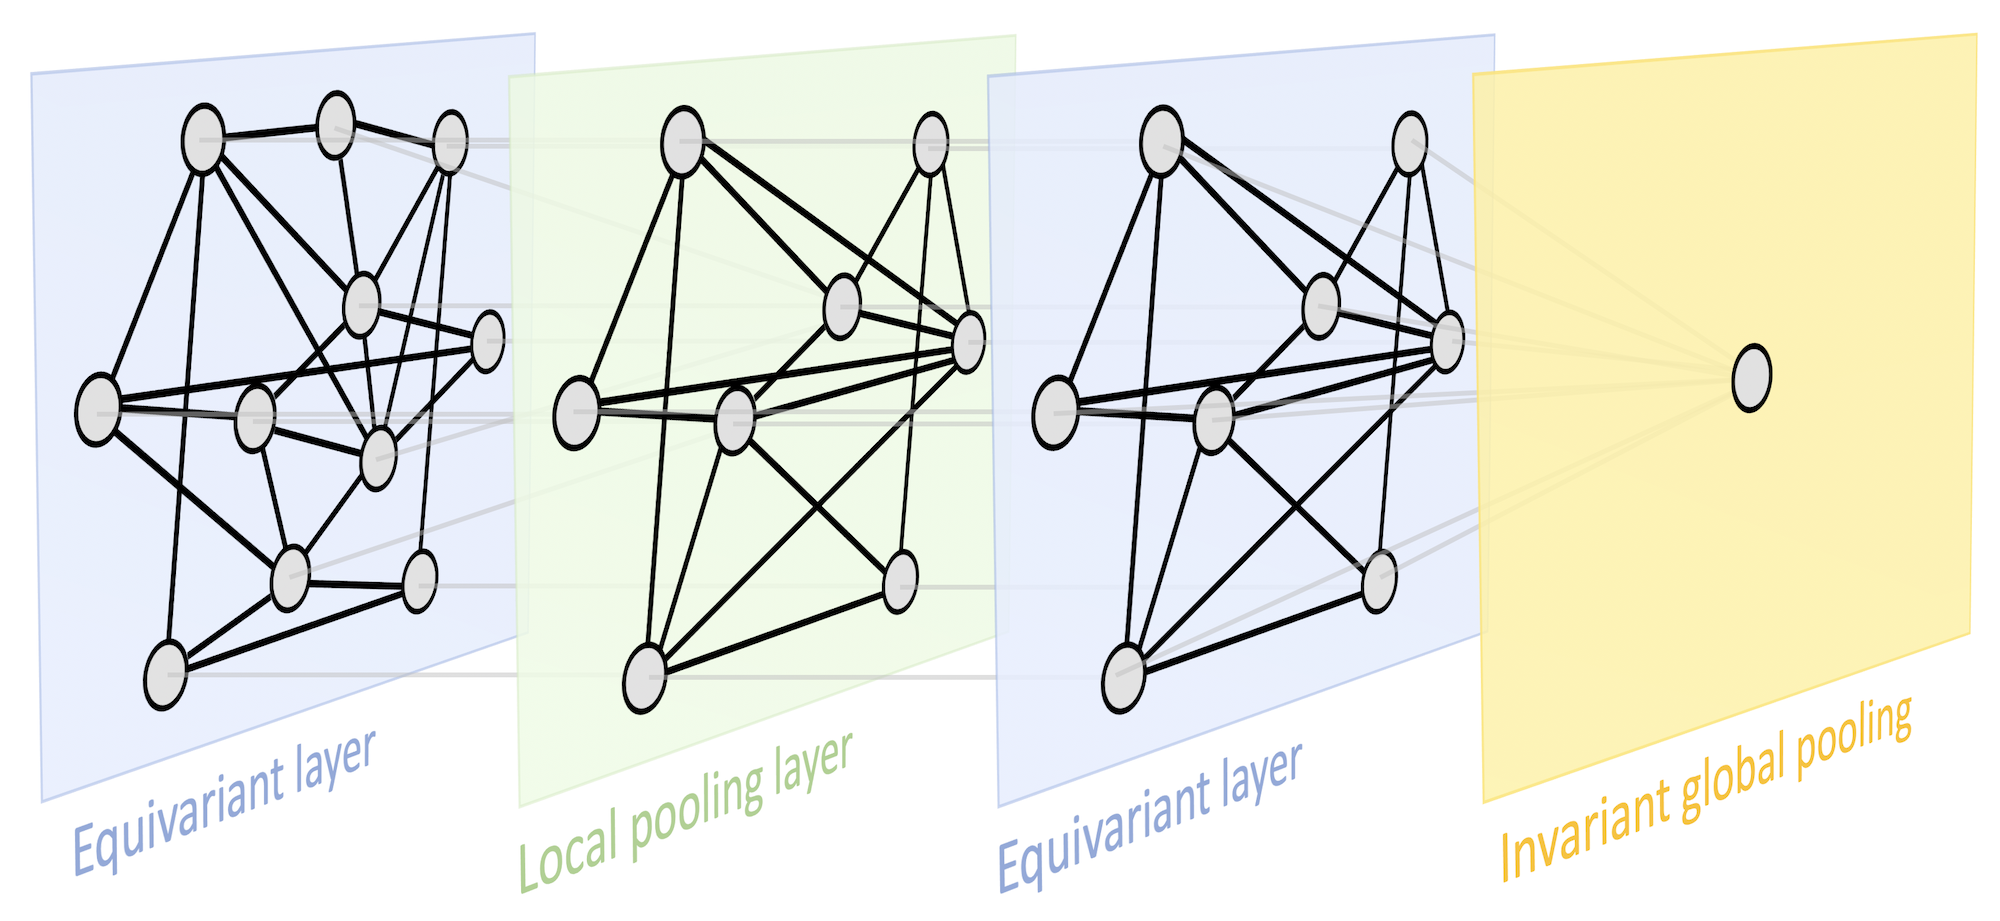
\includegraphics[width=1\textwidth]{figures/blueprint.png}
    \caption{以图为例说明的几何深度学习蓝图。典型的图神经网络架构可以包含置换等变层（计算逐节点特征）、局部池化（图粗化）以及置换不变的全局池化层（读出层）。}
    \label{fig:blueprint}
\end{figure}

总而言之，输入域的几何结构以及对其底层对称群的了解，给出了三个关键构件：（i）局部等变映射，（ii）全局不变映射，以及（iii）粗化算子。将这些构件组合在我们称为
%
\emph{几何深度学习蓝图}（图~\ref{fig:blueprint}）的方案中，即可得到一个具有预设不变性与稳定性性质的丰富函数逼近空间。
%
%We will see that a large number of popular neural network architectures used in deep representation learning are particular instances of this blueprint, illustrated in 
%across all the geometric domains we will describe next. 
%



%\begin{tcolorbox}[width=\linewidth,
%                  boxsep=0pt,
%                  left=7.5pt,
%                  right=7.5pt,
%                  top=7.5pt,
%                  bottom=7.5pt,
%                  arc=0pt,
%                  boxrule=0pt,toprule=0pt,
%                  colback=boxgray,
%                  ]%%
    
%\begin{center}
%Given a hierarchy of domains $\Omega_J \subseteq \hdots \subseteq \Omega_2 \subseteq \Omega_1 = \Omega$ with symmetry group $\fG$, the 
%\textbf{Geometric Deep Learning Blueprint} allows constructing $\fG$-invariant functions $f:\mathcal{X}(\Omega,\mathcal{C}) \rightarrow \mathcal{Y}$ of the form 
%$$
%f = A \circ \boldsymbol{\sigma}_J \circ U_J \circ P_{J-1} \circ \hdots \circ P_1 \circ \boldsymbol{\sigma}_1 \circ B_1
%$$
%consisting  of the following building blocks:\\

%    \noindent {\em Linear $\fG$-equivariant layer} $B_j: \gX(\Omega_j, \gC_j) \to \gX( \Omega_{j}, \gC'_{j})$ satisfying $B(\fg.x) = \fg.B(x)$ for all $\fg \in \fG$ and $x\in \gX(\Omega_j,\mathcal{C}_j)$. 
%    \vspace{2mm}\\

%    \noindent {\em Nonlinearity} $\sigma_j: \gC'_j \to \gC_j$ applied element-wise as $(\bm{\sigma}(x))(u) = \sigma( x(u))$.\vspace{2mm}\\\

%    \noindent {\em Local pooling (coarsening)}  $P_j : \gX(\Omega_j, \gC_j) \rightarrow \gX(\Omega_{j+1}, \gC_{j+1}) $.\vspace{2mm}\\
    
%    \noindent {\em Invariant layer (global pooling) } $A: \gX(\Omega_J, \gC_J) \rightarrow \mathcal{Y}$ satisfying $A(\fg .x) = A(x)$ for all $\fg \in \fG$ and $x\in \gX(\Omega_J,\mathcal{C}_J)$.  %.\vspace{2mm}\\

%\end{center}
%\end{tcolorbox}


\newpage
\begin{tcolorbox}[width=\linewidth,
                  boxsep=0pt,
                  left=7.5pt,
                  right=7.5pt,
                  top=4pt,
                  bottom=4pt,
                  arc=0pt,
                  boxrule=0pt,toprule=0pt,
                  colback=boxgray,
                  ]%%
\small
\begin{center}
\textbf{几何深度学习蓝图}
\end{center}
设 $\Omega$ 和 $\Omega'$ 为域，$\fG$ 为 $\Omega$ 上的对称群；我们用 $\Omega' \subseteq \Omega$ 表示 $\Omega'$ 可视为 $\Omega$ 的紧致版本。\\

我们定义如下构件：\vspace{2mm}\\

    \noindent {\em 线性 $\fG$-等变层} $B: \gX(\Omega, \gC) \to \gX( \Omega', \gC')$，满足 $B(\fg.x) = \fg.B(x)$，且该式对所有 $\fg \in \fG$ 和 $x\in \gX(\Omega,\mathcal{C})$ 均成立。\vspace{2mm}\\

    \noindent {\em 非线性} $\sigma: \gC \to \gC'$，按元素施加为 $(\bm{\sigma}(x))(u) = \sigma( x(u))$。\vspace{2mm}\\

    \noindent {\em 局部池化（粗化）} $P : \gX(\Omega, \gC) \rightarrow \gX(\Omega', \gC) $，其中 $\Omega'\subseteq\Omega$。\vspace{2mm}\\
    
    \noindent {\em $\fG$-不变层（全局池化）} $A: \gX(\Omega, \gC) \rightarrow \mathcal{Y}$，满足 $A(\fg .x) = A(x)$，且该式对所有 $\fg \in \fG$ 和 $x\in \gX(\Omega,\mathcal{C})$ 均成立。\vspace{2mm}\\

利用这些构件，可以构造如下形式的 $\fG$-不变函数 $f:\mathcal{X}(\Omega,\mathcal{C}) \rightarrow \mathcal{Y}$：
$$
f = A \circ \boldsymbol{\sigma}_J \circ B_J \circ P_{J-1} \circ \hdots \circ P_1 \circ \boldsymbol{\sigma}_1 \circ B_1
$$
其中，各构件的选择应使每个构件的输出空间与下一个构件的输入空间相匹配。不同构件可以利用不同的对称群 $\fG$ 选择。
\end{tcolorbox}

%


% A natural question is then how expressive this generic construction is in the class of $\fG$-invariant functions, and, equally important, which conditions on $B$ and $\rho$ ensure geometric stability.  
% Universal Approximation

% A simple option to ensure rich and stable representations is to instead compose several \emph{layers} of non-linear local equivariant maps before applying the global invariant. 

% The idea of deep learning is to define $f$ as a \emph{composition} of maps (or ``layers'').
% These maps should be compatible in that the output space of one layer should match the input space of the next layer.
% %That is, we can compose $f_1 : \mathcal{X}(\Omega, \mathcal{C}) \rightarrow \mathcal{X}(\Omega', \mathcal{C}')$ and $f_2 : \mathcal{X}(\Omega'', \mathcal{C}'') \rightarrow \mathcal{X}(\Omega''', \mathcal{C}''')$ if and only if $\mathcal{X}(\Omega', \mathcal{C}') = \mathcal{X}(\Omega'', \mathcal{C}'')$.
% That is, we can compose $f_1 : \mathcal{X}_1 \rightarrow \mathcal{X}_2$ and $f_2 : \mathcal{X}_2' \rightarrow \mathcal{X}_3$ if and only if $\mathcal{X}_2 = \mathcal{X}_2'$ (where we have abbreviated $\mathcal{X}_i = \mathcal{X}(\Omega_i, \mathcal{C}_i)$).
% Whereas in regular deep learning, maps can be composed as soon as the input and output spaces match as \emph{vector spaces} (i.e. they have the same dimensionality / array shape), in geometric deep learning these spaces should match as \emph{group representations}.
% This means that, in addition to matching as vector spaces, the group $\fG$ should act in the same way on both spaces.
% When this is the case, equivariance of $f_1$ and $f_2$ implies equivariance of the composition $f_2 \circ f_1$.

% Most networks in geometric deep learning are compositions of a few basic building blocks:

% %\emph{Local} 
% $\fG$-\emph{equivariant} linear operator $A: \gX(\Omega) \to \gX_{\gV'}(\Omega)$ satisfying $A(\fg.x) = \fg. A(x)$ for any $x \in \mathcal{X}(\Omega)$ and $\fg\in\fG$. 
% %
% Typically, this operator is further assumed to be {\em local}, i.e. $(Ax)(u)$ depends only on the values of $x(v)$ for $v$ in the vicinity of $u$, in the sense of some metric on $\Omega$.  
% %and such that $A x(u)$ only depends upon $\{ x(v); \mathrm{g}(v,u) \leq \delta\}$, where $\delta$ encodes the size of the neighborhood. 

% \emph{Pointwise nonlinearity} $\sigma: \mathcal{C}' \to \mathcal{C}''$. Under our assumptions, this implies that $\sigma \circ A$ is local and $\fG$-\emph{equivariant} whenever $A$ is such. \marginnote{When $\sigma$ acts coordinate-wise, it is typically referred to as an \emph{activation function}. In general,  $\sigma$ can be a generic function, such as a fully-connected neural network. }

% % \joan{
% % Argue that the only linear $\fG$-invariant is the group average. 
% % If $F$ is linear and $\fG$-invariant, then for all $x$, 
% % $$F(x) =  \frac{1}{\mu(\fG)} \int F( g.x) \mu(dg) = F\left(\frac{1}{\mu(\fG)} \int g.x \mu(dg) \right)~,$$
% % so $F$ only depends on $x$ through the average. 

% % This justifies why we need to add non-linearities
% % }




% {\em Local pooling} (or downsampling operator) $P_j: \gX(\Omega_j,\mathcal{C}_{j}) \to \gX(\Omega_{j+1},\mathcal{C}_{j+1})$ defined on a hierarchy of domains $\Omega_1, \hdots, \Omega_J$. 
% %reducing the resolution of the domain. 

% {\em Global pooling} $\fG$-{\em invariant} operator $a:\mathcal{X}(\Omega,\mathcal{C}) \rightarrow \mathcal{Y}$. 
    



% %
% %\michael{\bf [MB: INSERT FIGURE of a general equivariant/invariant architecture, similarly to Maron's thesis]}
% %
% %Let $\gX(\Omega, \gV) := \{ x : \Omega \to \gV \}$ be the input space, with domain $\Omega$ and feature space $\gV$ . We assume a metric $\mathrm{g}$ on $\Omega$ and a symmetry group $\fG$ acting on it, which also defines a linear representation 
% %%(taco confirm language? \taco{Correct. This is called the regular rep of G on X. Will add a definition to 1.2.1}) 
% %over $\gX$ by composition, as in Figure \ref{fig:symmetryactors}.
% %%if $x \in \gX$ and $g \in \fG$, then $g x (u) = x(gu) \in \R^s$. [we assume that the group does not act along channels for now]
% %\taco{TODO: add condition that signal space should have an inner product, i.e. be a Hilbert space. See definition box in 1.2}
% %
% %The GDL blueprint consists of four fundamental building blocks that are composed together appropriately:
% %\begin{enumerate}
% %    \item A \emph{local} $\fG$-\emph{equivariant} linear operator $A: \gX_{\gV}(\Omega) \to \gX_{\gV'}(\Omega)$; that is, $A(\fg.x) = \fg. A(x)$ for any $x$ and $\fg$, and such that $A x(u)$ only depends upon $\{ x(v); \mathrm{g}(v,u) \leq \delta\}$, where $\delta$ encodes the size of the neighborhood. 
% %    \item A \emph{nodewise} nonlinear activation function $\sigma: \gV' \to \gV''$. Under our assumptions, this implies that $\sigma \circ A$ is local and $\fG$-\emph{equivariant} whenever $A$ is as above. When $\text{dim}(\gV')=\text{dim}(\gV'')=1$, $\sigma$ is typically described as an \emph{activation function}, but in general $\sigma$ can be a generic function, such as a fully-connected neural network. 
% %    \item Local pooling or downsampling operator $P_k: \gX_{\gV}(\Omega_k) \to \gX_{\gV}(\Omega_{k+1})$ reducing the resolution of the domain. 
% %    \item Global pooling: $\fG$-invariant operator. 
% %\end{enumerate}




% %\michael{MB: I am in favor of keeping the blueprint as simple as possible even at the expense of precision of definitions/generality. It should be intuitive and I feel currently the intuition is buried under too much notation. }


% The majority of deep neural networks implement a composition of multiple such components of the form
% $$
% f =a \circ P_L \circ \sigma_L \circ A_L \dots P_1 \circ \sigma_1 \circ A_1,
% $$
% with each component referred to as a {\em layer}. The term `deep' is used to indicate that there are many such layers, though we should say that how deep is deep is in the eyes of the beholder.\marginnote{Some CNN architectures used in computer vision can have hundreds of layers. }
% %
% %The multilayer composition $f =a \circ P_L \circ \sigma_L \circ A_L \dots P_1 \circ \sigma_1 \circ A_1$ 
% %
% Such a multilayer construction allows to define a flexible functional space with prescribed geometric priors. On the one hand, the equivariant nature of the maps $\sigma \circ A_j$ is preserved under composition, resulting in overall invariance when composed with a global pooling operator. On the other hand, the use of pooling layers allows to exploit the scale separation prior. 

\paragraph{几何深度学习的不同设定}
这里可以作出一个重要区分：一种设定假定域 $\Omega$ {\em 固定}，仅关注定义在该域上的可变输入信号；另一种设定则将域作为输入的一部分，使其与定义于其上的信号一同{\em 变化}。
%
前一种情形的经典实例见于计算机视觉应用，其中图像被假定定义在固定域（网格）上。
%
图分类是后一种设定的例子，其中图的结构及定义在其上的信号（例如节点特征）都很重要。
%
在域可变的情形下，几何稳定性（即对 $\Omega$ 形变的不敏感性）在几何深度学习架构中起着关键作用。


该蓝图具有恰当的普适程度，可用于广泛的几何域。
因此，不同的几何深度学习方法在域、对称群的选择以及上述构件的具体实现细节上有所不同。
%and the metric defining locality. 
正如下文将看到的，目前使用的一大类深度学习架构都属于这一方案，因而可以从共同的几何原理导出。
%
%We will now discuss specific instances of this blueprint and how it adapts to each case.  


在以下各节（\ref{sec:proto-graphs}--\ref{sec:meshes}）中，我们将以“5G”为重点介绍各种几何域；在第~\ref{sec:cnnsec}--\ref{sec:lstm} 节中，则介绍几何深度学习在这些域上的具体实现。



%Such generic architecture, illustrated in Figure~\ref{fig:blueprint}, can be instantiated across a variety of domains with different geometric structures giving rise to a very large zoo of architectures united by these common geometric principles. Let us now discuss these domains and how this blueprint adapts to each case. 


% First, we define a collection of \emph{local} $\fG$-\emph{equivariant} linear operators. In  deep learning architectures such as CNNs and GNNs these correspond to convolutional and message passing layers, and the corresponding groups are translation and permutation, respectively. 

% Next, these operators are composed with a non-linearity called an {\em activation function} in the neural networks jargon, which preserves the equivariance as it is applied element-wise. \taco{TC: note that element-wise nonlinearities are only equivariant to certain kinds of group representations, namely when the representation matrices are all permutation matrices}

% Finally, coarsen the representations produced by the equivariant operators. In image analysis applications, this is achieved by means of {\em pooling}, an operation reducing the size of the image grid, and as we shall see next, coarsening may be defined on far more general data domains.

% In an idealised instantiation, the coarsening is performed at the output. It can be shown that this representation is 
% provably $\fG$-invariant/equivariant, and that the locality assumption captures the scale separation inductive bias. 
% Moreover, such representations are universal approximators under symmetry, as we discuss in Chapter ??. 

%\joan{Joan: Taco, we can generalise the blueprint to accommodate more group representations, if we feel the use cases are sufficiently important. Otherwise, an alternative is to mention that this blueprint can be extended in some domains to account for special types of group actions}

%\taco{Taco: Joan, I agree we really only need reps that describe how signals transform. However that is still a bit more general than $\rho(\fg) x(u) = x(\fg^{-1} u)$. In particular for steerable cnns / induced reps, as well as gauge cnns, we have some smaller group acting on the feature vector. E.g. a vector field on the sphere transforms according to the rep of SO3 that is induced by the vector rep of SO2 acting on 2D vectors. 

%One option is to ignore this for now and call this the ``deep learning blueprint (simplified)'', and mention that we need something slightly more general. We can introduce the full thing in a separate chapter. Only downside is that we cannot write the gauges section of the intro to conform to the simplified blueprint then. May not be such a big deal...

%Alternatively, we can first introduce a general definition for arbitrary reps, then introduce one specialized version for $\rho(\fg) x(u) = x(\fg^{-1} u)$. Then later we can say in the gauges section that the gauge story fits the general blueprint but involves a different kind of rep.
%}


%(either explicitly or implictly since energy is pushed towards low frequencies).
    

%\begin{enumerate}
%    \item Define a collection of \emph{local}, $\gG$-\emph{equivariant} linear operators $U_m$. 
%    \item Compose them with an element-wise non-linearity $\rho$. 
%    \item Coarsen the hidden representations (either explicitly or %implictly since energy is pushed towards low frequencies).
%\end{enumerate}





\begin{tcolorbox}[width=\linewidth,
                  boxsep=0pt,
                  left=7.5pt,
                  right=7.5pt,
                  top=7.5pt,
                  bottom=7.5pt,
                  arc=0pt,
                  boxrule=0pt,toprule=0pt,
                  colback=boxgray,
                  ]%%
    
\begin{center}
%\textbf{Geometric Deep Learning Blueprint}\newline
\begin{tabular}{lll}
     {\bf 架构} & {\bf 域} $\Omega$ & {\bf 对称群} $\mathfrak{G}$\vspace{2.5mm}\\
     {\em CNN} & 网格 & 平移\vspace{2mm}\\
%
     {\em 球面 CNN} & 球面 / $\mathrm{SO}({3})$ & 旋转 $\mathrm{SO}({3})$\vspace{2mm}\\

     {\em 内蕴 / 网格 CNN} & 流形 & 等距变换 $\mathrm{Iso}(\Omega)$ / \\
     & & 规范对称性 $\mathrm{SO}(2)$\vspace{2mm}\\


     {\em GNN} & 图 & 置换 $\Sigma_n$\vspace{2mm}\\

     {\em Deep Sets} & 集合 & 置换 $\Sigma_n$\vspace{2mm}\\
     {\em Transformer} & 完全图 & 置换 $\Sigma_n$\vspace{2mm}\\
     {\em LSTM} & 一维网格 & 时间扭曲\\


\end{tabular}
\end{center}
\end{tcolorbox}
%

%\begin{tcolorbox}[width=\linewidth,
%                  boxsep=0pt,
%                  left=7.5pt,
%                  right=7.5pt,
%                  top=7.5pt,
%                  bottom=7.5pt,
%                  arc=0pt,
%                  boxrule=0pt,toprule=0pt,
%                  colback=boxgray,
%                  ]%%
%    
%\begin{center}
%\textbf{Geometric Deep Learning Blueprint instances of interest}\newline
%\begin{tabular}{cccc}
%     Domain, $\Omega$ & Metric, $g$ & Symmetry group, $\frak{G}$ & Architecture\\
%     {\bf Grids} & $L_\infty$ & Translations & {\bf CNNs}\\ 
%     {\bf Spheres} & Great circle & \multirow{2}{*}{3D rotations, SO(3)} & \multirow{2}{*}{\bf Spherical CNNs} \\
%     {\bf SO(3)} & Geodesic & \\
%     \multirow{2}{*}{\bf Gauges} & \multirow{2}{*}{Geodesic} & \multirow{2}{*}{\{Gauge transform.\}} & {\bf Gauge Equivariant} \\ & & & {\bf Mesh CNNs} \\
%     {\bf Graphs} & Shortest path & Permutations, $\Sigma_n$ & {\bf GNNs}\\
%     \multirow{2}{*}{\bf Sets} & $+\infty$ & Permutations, $\Sigma_n$ & {\bf Deep Sets}\\
%     & $0$ & Permutations, $\Sigma_n$ & {\bf Transformers}\\
%\end{tabular}
%\end{center}
%\end{tcolorbox}


%\begin{figure}
%    \centering
%    \includegraphics[width=0.9\textwidth]{figures/equivariant-network-blueprint.png}
%    \caption{todo}
%    \label{fig:equivariant-net-blueprint}
%\end{figure}




%\michael{\bf [MB: give examples here?]}



%{\bf 
%Main questions:

%What the equivariant structure that is required at every hidden %layer. 
%Universality vs efficiency. 

%Generalization?
%}

%Scale separation in neural networks

%Graph isomorphism Gromov graphs

%Link to deformation stability. 

%\subsection{{Leveraging Geometric Structure}}

% \begin{itemize}
%     \item Two main universal principles: symmetries and scale separation. 
%     \item These two principles have deep long roots in physics and mathematics (homogeneization, Galois theory, Noether's theorem, etc etc etc)
%     \item They are omnipresent in many modern data domains: computer vision, physical systems, chemistry, networks.  
%     \item Can we make these principles compatible with large scale ML models (gradient-based learning)? 
%     \item Can we recover Universal approximation models while leveraging geometric structure. It turns out that Neural Networks are a good language for that since we can add symmetry and scale while preserving their universal approximation properties. 
% \end{itemize}
